\documentclass[t,aspectratio=169,xcolor=dvipsnames]{beamer}

\usepackage{hyperref}
\usepackage{graphicx}
\usepackage{booktabs}
\usepackage{tikz}
\usetikzlibrary{shapes,arrows,arrows.meta,positioning,calc,matrix,fit,backgrounds,decorations.pathreplacing}
\usepackage{pgfplots}
\pgfplotsset{compat=1.18}
\usepackage{makecell}
\usepackage{setspace}
\usepackage[utf8]{inputenc}
\usepackage[T1]{fontenc}
\usepackage{helvet}
\usepackage{amsmath,amssymb,amsfonts}
\usepackage{bm}
\usepackage{ragged2e}
\usepackage{listings}
\usepackage{xcolor}

% --- Minimalist Color Palette (DESIGN.md) ---
\definecolor{dlInk}{HTML}{111111}
\definecolor{dlCanvas}{HTML}{FFFFFF}
\definecolor{dlSoftCloud}{HTML}{F5F5F5}
\definecolor{dlCharcoal}{HTML}{39393B}
\definecolor{dlMute}{HTML}{707072}
\definecolor{dlHairline}{HTML}{CACACB}
\definecolor{dlTeal}{HTML}{0A7281}
\definecolor{dlBlue}{HTML}{1151FF}
\definecolor{dlOrange}{HTML}{DE8F05}
\definecolor{codeBg}{HTML}{F7F7F8}
\newcommand{\con}[1]{\textcolor{dlOrange}{#1}}

% --- Beamer Theme Customization ---
\usetheme{default}
\useinnertheme{rectangles}
\setbeamertemplate{navigation symbols}{}

\setbeamercolor{palette primary}{bg=dlInk,fg=dlCanvas}
\setbeamercolor{palette secondary}{bg=dlCharcoal,fg=dlCanvas}
\setbeamercolor{palette tertiary}{bg=dlSoftCloud,fg=dlInk}
\setbeamercolor{structure}{fg=dlInk}
\setbeamercolor{title}{fg=dlCanvas,bg=dlInk}
\setbeamercolor{frametitle}{fg=dlInk,bg=dlSoftCloud}
\setbeamercolor{normal text}{fg=dlInk,bg=dlCanvas}
\setbeamercolor{block title}{bg=dlInk,fg=dlCanvas}
\setbeamercolor{block body}{bg=dlSoftCloud,fg=dlInk}
\setbeamercolor{block title example}{bg=dlTeal,fg=dlCanvas}
\setbeamercolor{block body example}{bg=dlSoftCloud,fg=dlInk}
\setbeamercolor{block title alert}{bg=dlCharcoal,fg=dlCanvas}
\setbeamercolor{block body alert}{bg=dlSoftCloud,fg=dlInk}
\setbeamercolor{item}{fg=dlInk}

\makeatletter
\setbeamertemplate{frametitle}{%
  \nointerlineskip%
  \begin{beamercolorbox}[wd=\paperwidth,ht=3.8ex,dp=1.5ex,leftskip=1.0cm,rightskip=1.0cm]{frametitle}%
    \textbf{\large\strut\insertframetitle}%
    \ifx\insertframesubtitle\@empty\else\hfill{\footnotesize\color{dlMute}\insertframesubtitle}\fi%
  \end{beamercolorbox}%
}
\makeatother

\setbeamertemplate{footline}{%
  \begin{beamercolorbox}[wd=\paperwidth,ht=2.5ex,dp=1.2ex,leftskip=1.0cm,rightskip=1.0cm]{palette primary}%
    \tiny\textbf{IF25-40401 · Deep Learning} \hfill \insertshorttitle \hfill \textbf{\insertframenumber{} / \inserttotalframenumber}%
  \end{beamercolorbox}%
}

\lstset{
  backgroundcolor=\color{codeBg},
  basicstyle=\ttfamily\scriptsize\color{dlInk},
  keywordstyle=\bfseries\color{dlTeal},
  commentstyle=\color{dlMute}\itshape,
  stringstyle=\color{dlCharcoal},
  breaklines=true,
  frame=single,
  rulecolor=\color{dlHairline},
  numbers=none,
  tabsize=2,
  showstringspaces=false
}

\lstdefinestyle{py}{
  language=Python,
  basicstyle=\ttfamily\fontsize{6.8pt}{8.2pt}\selectfont\color{dlInk},
  keywordstyle=\bfseries\color{dlTeal},
  commentstyle=\color{dlMute}\itshape,
  stringstyle=\color{dlCharcoal},
  columns=fullflexible,
  keepspaces=true
}

% --- TikZ styles ---
\tikzset{
  lyr/.style={draw=dlInk, fill=dlSoftCloud, rounded corners=2pt, minimum height=0.55cm, inner sep=3pt, font=\scriptsize, align=center},
  lyrT/.style={lyr, fill=dlTeal!15, draw=dlTeal},
  lyrB/.style={lyr, fill=dlBlue!10, draw=dlBlue},
  lyrO/.style={lyr, fill=dlOrange!15, draw=dlOrange},
  arr/.style={-{Stealth[length=4pt]}, thick, draw=dlCharcoal},
  addn/.style={circle, draw=dlInk, thick, inner sep=0pt, minimum size=0.45cm, font=\small},
}

% --- Section divider macro ---
\newcommand{\bagian}[3]{%
\begin{frame}[plain]
  \begin{beamercolorbox}[wd=\paperwidth,ht=\paperheight,sep=1.5cm]{palette primary}
    \vspace{1.5cm}
    {\scriptsize\bfseries\color{dlMute}#1}\\[0.4cm]
    {\Huge\bfseries #2}\\[0.4cm]
    {\small\color{dlHairline}#3}
    \vfill
  \end{beamercolorbox}
\end{frame}}

\title[Pertemuan 5: CNN dan Variasinya]{Deep Learning (IF25-40401)}
\subtitle{Pertemuan 5: CNN dan Variasinya}
\author{Tim Dosen Deep Learning}
\institute{Teknik Informatika — Institut Teknologi Sumatera (ITERA)}
\date{2026}

\begin{document}

% --- TITLE SLIDE ---
\begin{frame}[plain]
  \begin{beamercolorbox}[wd=\paperwidth,ht=\paperheight,sep=1.5cm]{palette primary}
    \vspace{0.8cm}
    {\scriptsize\bfseries\color{dlMute}IF25-40401 · DEEP LEARNING · PERTEMUAN 05}\\[0.4cm]
    {\Huge\bfseries DEEP COMPUTER VISION (2):\\CNN DAN VARIASINYA}\\[0.4cm]
    {\small AlexNet, VGG, GoogLeNet, ResNet, MobileNet, EfficientNet, ConvNeXt, dan Deteksi/Segmentasi}\\[1.0cm]
    \vfill
    {\scriptsize\textbf{Tim Dosen Deep Learning} · Institut Teknologi Sumatera (ITERA)}
  \end{beamercolorbox}
\end{frame}

%------------------------------------------------
\begin{frame}[plain]
    \frametitle{TUJUAN PEMBELAJARAN}
    \framesubtitle{Capaian Pembelajaran Pertemuan 5 (RPS IF25-40401)}

    \begin{exampleblock}{Setelah mengikuti pertemuan ini, mahasiswa diharapkan mampu:}
        \begin{enumerate}
            \item \textbf{Menjelaskan evolusi CNN dari AlexNet menuju VGG}
            \item \textbf{Menjelaskan desain blok konvolusi berlapis} ($3\times3$ bertumpuk) pada VGG
            \item \textbf{Menjelaskan residual connection} dan alasan ResNet bisa jauh lebih dalam
            \item \textbf{Membandingkan efisiensi MobileNet} (depthwise separable) dengan CNN standar
            \item \textbf{Mengidentifikasi elemen modern ConvNeXt} yang diadopsi dari Transformer
            \item \textbf{Menjelaskan prinsip object detection dan segmentasi} sebagai perluasan CNN
        \end{enumerate}
    \end{exampleblock}
\end{frame}

%------------------------------------------------
\begin{frame}[plain]
    \frametitle{OUTLINE}
    \framesubtitle{~}
    \begin{spacing}{1.2}
        \tableofcontents
    \end{spacing}
\end{frame}

%------------------------------------------------
\begin{frame}
    \frametitle{Dari LeNet-5 ke Arsitektur Modern}
    \framesubtitle{Jembatan dari Pertemuan 4}
    \footnotesize

    \begin{alertblock}{Temuan Notebook 03 (Pertemuan 4)}
        LeNet-5 mencapai $>98\%$ pada MNIST, tetapi \textbf{mentok di kisaran $\sim$60\% pada CIFAR-10}: kapasitas kecil (6/16 filter), hanya 2 layer konvolusi, tanpa BatchNorm/Dropout/augmentasi.
    \end{alertblock}

    \textbf{Pertanyaan hari ini:} bagaimana CNN menjadi \textbf{lebih dalam}, \textbf{lebih efisien}, dan \textbf{lebih serbaguna}?

    \vspace{0.3cm}
    \begin{center}
    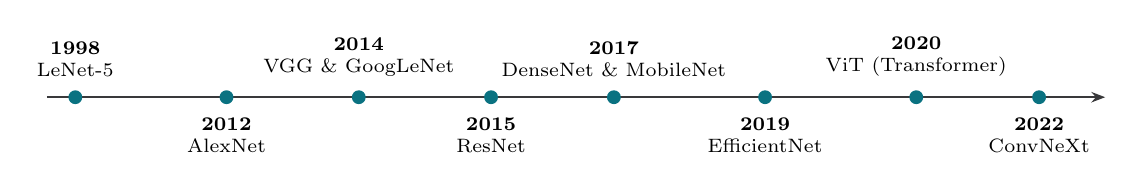
\begin{tikzpicture}[x=1.2cm]
        \draw[-{Stealth[length=5pt]}, thick, dlCharcoal] (0,0) -- (11.2,0);
        \foreach \x/\yr/\nm/\pos in {0.3/1998/LeNet-5/above, 1.9/2012/AlexNet/below, 3.3/2014/VGG \& GoogLeNet/above, 4.7/2015/ResNet/below, 6.0/2017/DenseNet \& MobileNet/above, 7.6/2019/EfficientNet/below, 9.2/2020/ViT (Transformer)/above, 10.5/2022/ConvNeXt/below}{
            \fill[dlTeal] (\x,0) circle (2.5pt);
            \node[\pos=4pt, font=\scriptsize, align=center] at (\x,0) {\textbf{\yr}\\\nm};
        }
    \end{tikzpicture}
    \end{center}

    \vspace{0.1cm}
    {\scriptsize\color{dlMute} Tiga tema besar: \textbf{kedalaman} (AlexNet $\to$ VGG $\to$ ResNet) · \textbf{efisiensi} (GoogLeNet, MobileNet, EfficientNet) · \textbf{desain modern} (ConvNeXt).}
\end{frame}

%================================================
\section{Era ImageNet: AlexNet \& VGG}
\bagian{BAGIAN 01 · ERA IMAGENET}{AlexNet \& VGG}{Lebih Dalam, Lebih Besar, dan Dilatih dengan GPU}

%------------------------------------------------
\begin{frame}
    \frametitle{ImageNet \& Kompetisi ILSVRC}
    \framesubtitle{Benchmark yang Memicu Revolusi}
    \footnotesize

    \begin{columns}[T]
        \column{0.40\textwidth}
        \begin{block}{ILSVRC (2010--2017)}
            \begin{itemize}
                \item $\pm$1,2 juta citra latih, \textbf{1.000 kelas}
                \item Metrik: \textbf{top-5 error}
            \end{itemize}
        \end{block}
        \begin{itemize}
            \item \textbf{2012:} AlexNet memangkas error $\sim$10 poin sekaligus.
            \item Sejak itu seluruh pemenang adalah \textbf{CNN}.
            \item 2015: ResNet melampaui estimasi manusia ($\sim$5,1\%).
        \end{itemize}

        \column{0.56\textwidth}
        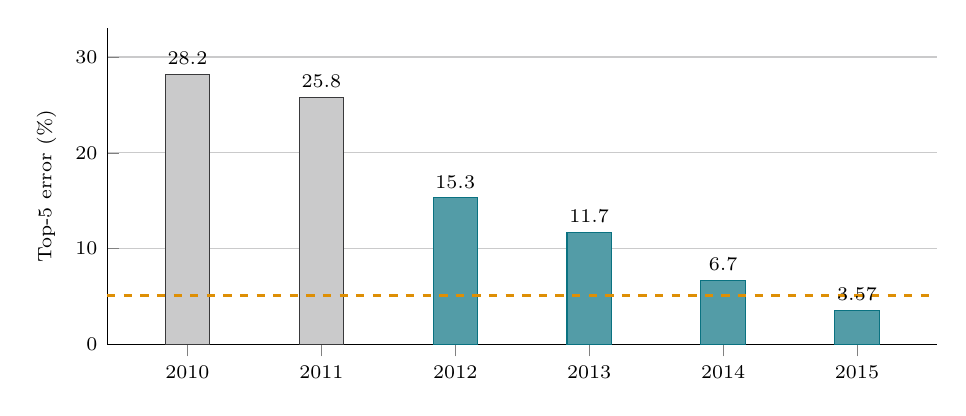
\begin{tikzpicture}
        \begin{axis}[
            ybar, bar width=16pt, width=\linewidth, height=5.6cm,
            ymin=0, ymax=33, ylabel={Top-5 error (\%)},
            symbolic x coords={2010,2011,2012,2013,2014,2015},
            xtick={2010,2011,2012,2013,2014,2015}, xticklabel style={font=\scriptsize}, yticklabel style={font=\scriptsize},
            ylabel style={font=\scriptsize},
            nodes near coords, every node near coord/.append style={font=\scriptsize},
            axis lines*=left, ymajorgrids, grid style={dlHairline},
            enlarge x limits=0.12,
        ]
            \addplot[fill=dlHairline, draw=dlCharcoal, bar shift=0pt] coordinates {(2010,28.2) (2011,25.8)};
            \addplot[fill=dlTeal!70, draw=dlTeal, bar shift=0pt] coordinates {(2012,15.3) (2013,11.7) (2014,6.7) (2015,3.57)};
            \draw[dashed, thick, dlOrange] (rel axis cs:0,0.155) -- (rel axis cs:1,0.155);
        \end{axis}
        \end{tikzpicture}
        {\scriptsize\color{dlMute} 2010 NEC · 2011 XRCE · 2012 AlexNet · 2013 ZFNet · 2014 GoogLeNet · 2015 ResNet · \textcolor{dlOrange}{garis putus-putus: estimasi manusia $\approx$5,1\%}}
    \end{columns}
\end{frame}

%------------------------------------------------
\begin{frame}
    \frametitle{AlexNet (2012): Tim SuperVision}
    \framesubtitle{Krizhevsky, Sutskever \& Hinton}
    \footnotesize

    \begin{columns}[T]
        \column{0.36\textwidth}
        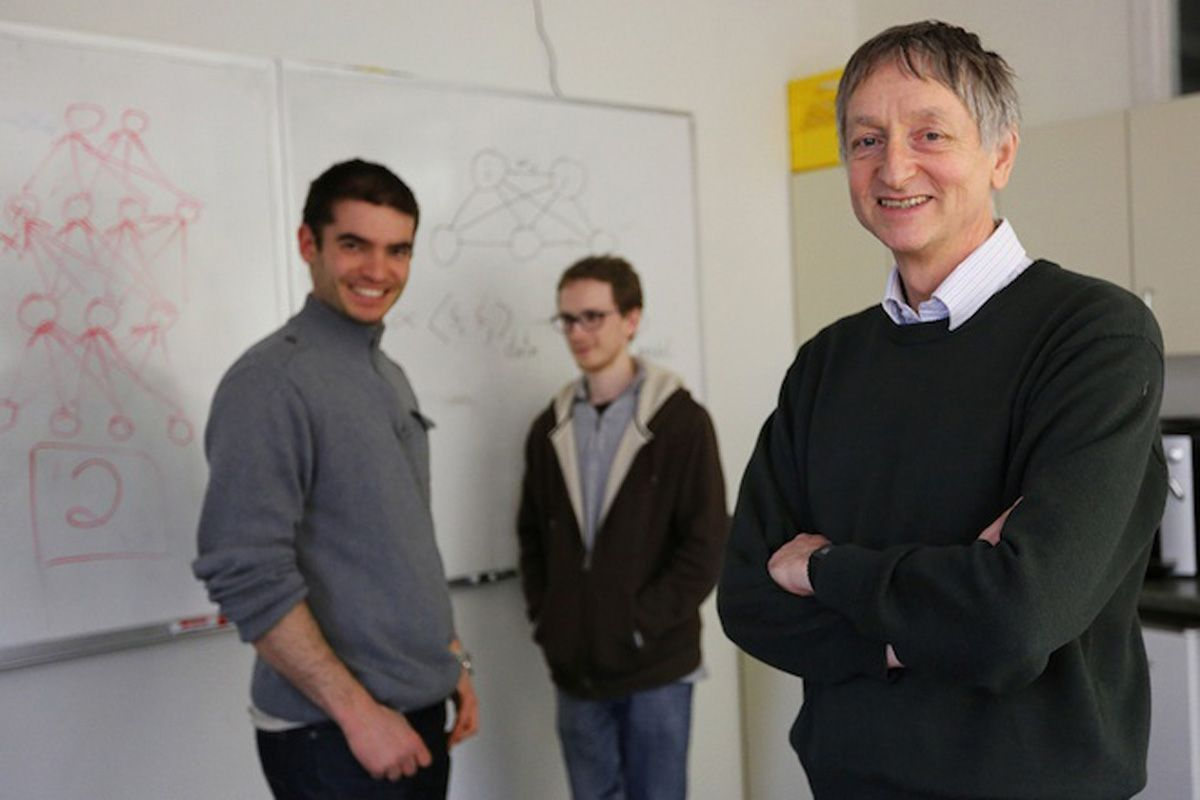
\includegraphics[width=0.8\linewidth]{figures/alex_ilya_geofrey.jpg}\\
        {\scriptsize\textcolor{gray}{Credit: University of Toronto / Wired}}

        \vspace{0.2cm}
        \begin{itemize}
            \item Top-5 error \textbf{15,3\%} vs 26,2\%
            \item 5 conv + 3 FC $=$ \textbf{8 layer}
            \item $\sim$6 hari di \textbf{2 GPU GTX 580}
        \end{itemize}

        \column{0.60\textwidth}
        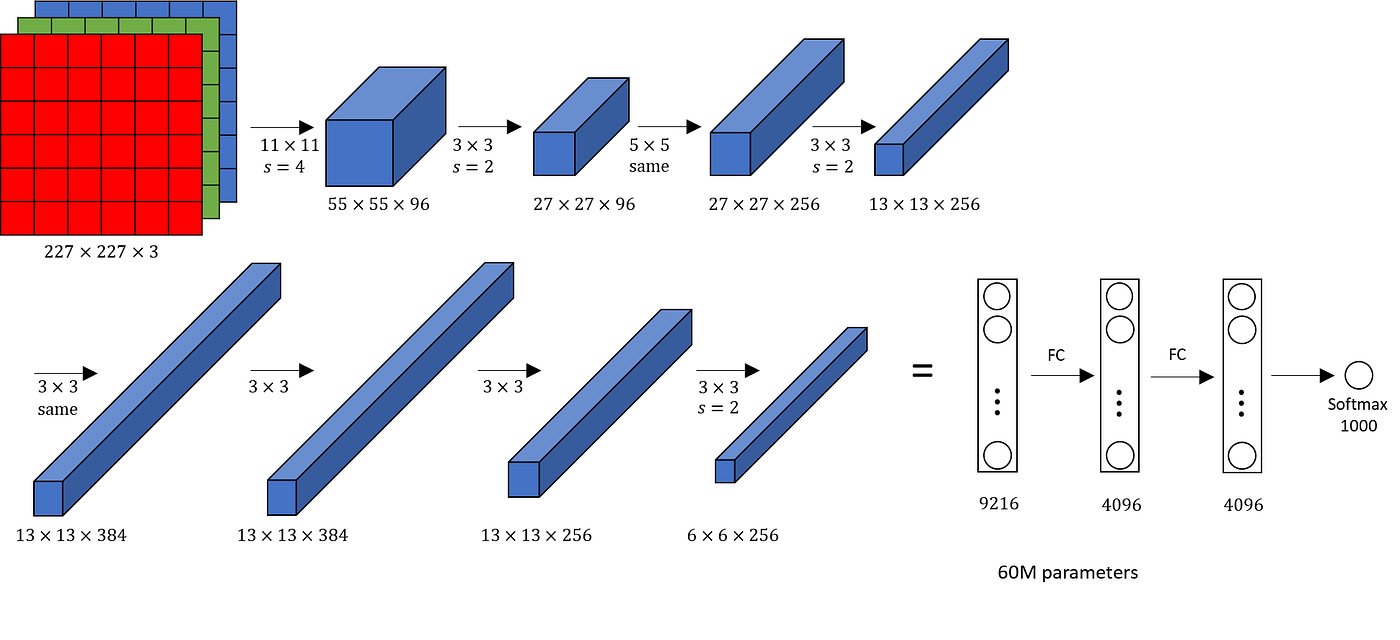
\includegraphics[width=\linewidth]{figures/4_alexnet_arch.png}\\
        {\scriptsize\textcolor{gray}{Credit: Krizhevsky et al. (2012), diolah ulang}}

        \vspace{0.2cm}
        Arsitektur terbelah dua jalur karena model tidak muat di memori satu GPU --- ide yang kelak kembali sebagai \textbf{grouped convolution}.
    \end{columns}
\end{frame}

%------------------------------------------------
\begin{frame}
    \frametitle{Menelusuri Dimensi \& Parameter AlexNet}
    \framesubtitle{Menerapkan Rumus Pertemuan 4}
    \footnotesize
    \vspace{2pt}
    \begin{columns}[T]
        \column{0.48\textwidth}
        \scriptsize\setlength{\tabcolsep}{3.5pt}
        \begin{tabular}{llrr}
            \toprule
            \textbf{Layer} & \textbf{Konfigurasi} & \textbf{Output} & \textbf{Param} \\
            \midrule
            Input & RGB & $227^2\times3$ & -- \\
            Conv1 & 96, $11\times11$, $S{=}4$ & $55^2\times96$ & 34.944 \\
            MaxPool & $3\times3$, $S{=}2$ & $27^2\times96$ & 0 \\
            Conv2 & 256, $5\times5$, $P{=}2$ & $27^2\times256$ & 614.656 \\
            MaxPool & $3\times3$, $S{=}2$ & $13^2\times256$ & 0 \\
            \bottomrule
        \end{tabular}
        \column{0.48\textwidth}
        \scriptsize\setlength{\tabcolsep}{3.5pt}
        \begin{tabular}{llrr}
            \toprule
            \textbf{Layer} & \textbf{Konfigurasi} & \textbf{Output} & \textbf{Param} \\
            \midrule
            Conv3--5 & 384/384/256, $3{\times}3$ & $13^2\times256$ & 3,7 jt \\
            MaxPool & $3\times3$, $S{=}2$ & $6^2\times256$ & 0 \\
            FC6 & 9216 $\to$ 4096 & 4096 & 37,8 jt \\
            FC7 & 4096 $\to$ 4096 & 4096 & 16,8 jt \\
            FC8 & 4096 $\to$ 1000 & 1000 & 4,1 jt \\
            \bottomrule
        \end{tabular}
    \end{columns}
    \vspace{0.3cm}
    \begin{columns}[T]
        \column{0.44\textwidth}
        \begin{exampleblock}{Contoh: Output Conv1}
            $$W_{out}=\left\lfloor\frac{227-11+2\cdot0}{4}\right\rfloor+1=\mathbf{55}$$
        \end{exampleblock}
        \column{0.52\textwidth}
        \begin{itemize}
            \item Total $\approx$ \textbf{61 juta} parameter --- $\sim$1000$\times$ LeNet-5 (61.706).
            \item \textbf{$\sim$96\%} parameter ada di FC6--FC8 (58,6 juta), pola yang sama dengan LeNet-5.
            \item FC6 saja: $(6\cdot6\cdot256+1)\times4096 = 37{,}8$ juta.
        \end{itemize}
    \end{columns}
\end{frame}

%------------------------------------------------
\begin{frame}
    \frametitle{Empat Kunci Keberhasilan AlexNet}
    \framesubtitle{Bukan Hanya Soal Kedalaman}
    \footnotesize

    \begin{columns}[T]
        \column{0.48\textwidth}
        \textbf{1. Aktivasi ReLU} $\;f(x)=\max(0,x)$
        \begin{itemize}
            \item Sigmoid: $\sigma'(x)\le 0{,}25$ $\Rightarrow$ gradien mengecil tiap layer (\textit{vanishing gradient}).
            \item ReLU: turunan $=1$ untuk $x>0$ $\Rightarrow$ konvergensi $\sim$6$\times$ lebih cepat daripada tanh.
        \end{itemize}
        \textbf{2. Dropout} ($p=0{,}5$ di FC6 \& FC7)
        \begin{itemize}
            \item Mematikan neuron acak saat training $\Rightarrow$ mencegah ko-adaptasi, menekan overfitting 58 juta bobot FC.
        \end{itemize}

        \column{0.48\textwidth}
        \textbf{3. Augmentasi Data}
        \begin{itemize}
            \item Random crop $224\times224$ dari $256\times256$ + horizontal flip ($\sim$2048$\times$ variasi).
            \item Perturbasi warna berbasis PCA pada kanal RGB.
        \end{itemize}
        \textbf{4. Training di GPU}
        \begin{itemize}
            \item Konvolusi paralel di CUDA; model dibagi ke 2 GPU.
            \item Bukti bahwa \textbf{data besar + GPU} membuka jalan deep learning.
        \end{itemize}
        \vspace{0.1cm}
        {\scriptsize\color{dlMute} (Juga: Local Response Normalization \& overlapping pooling --- kini sudah ditinggalkan.)}
    \end{columns}
\end{frame}

%------------------------------------------------
\begin{frame}
    \frametitle{LeNet-5 vs AlexNet: Lompatan Generasi}
    \framesubtitle{14 Tahun, Skala Berubah Total}
    \footnotesize
    \vspace{4pt}
    \begin{center}
    \begin{tabular}{lll}
        \toprule
        \textbf{Aspek} & \textbf{LeNet-5 (1998)} & \textbf{AlexNet (2012)} \\
        \midrule
        Layer terlatih & 5 (2 conv + 3 FC) & 8 (5 conv + 3 FC) \\
        Parameter & 61.706 & $\sim$61 juta \\
        Input & $32\times32\times1$ & $227\times227\times3$ \\
        Aktivasi & Tanh & \textbf{ReLU} \\
        Pooling & Average $2\times2$ & Max $3\times3$, stride 2 (overlap) \\
        Regularisasi & -- & \textbf{Dropout + augmentasi} \\
        Dataset & MNIST (60 ribu, 10 kelas) & ImageNet (1,2 juta, 1000 kelas) \\
        Perangkat & CPU & 2$\times$ GPU GTX 580 \\
        \bottomrule
    \end{tabular}
    \end{center}
    \vspace{0.2cm}
    \textbf{Takeaway:} ide dasarnya sama (\textit{conv $\to$ pool $\to$ FC}); yang berubah adalah \textbf{skala data, komputasi, dan trik pelatihan}.
\end{frame}

%------------------------------------------------
\begin{frame}[fragile]
    \frametitle{AlexNet di PyTorch}
    \framesubtitle{Blok Ekstraktor Fitur Pertama}
    \footnotesize

    \begin{columns}[T]
        \column{0.60\textwidth}
\begin{lstlisting}[style=py]
import torch.nn as nn
from torchvision import models

features = nn.Sequential(
    nn.Conv2d(3, 64, kernel_size=11, stride=4, padding=2),
    nn.ReLU(inplace=True),                 # bukan Tanh
    nn.MaxPool2d(kernel_size=3, stride=2), # overlapping
    nn.Conv2d(64, 192, kernel_size=5, padding=2),
    nn.ReLU(inplace=True),
    # ... conv3-conv5, lalu AdaptiveAvgPool2d((6, 6))
)
alexnet = models.alexnet(weights="IMAGENET1K_V1")
\end{lstlisting}

        \column{0.36\textwidth}
        \begin{itemize}
            \item Versi torchvision memakai 64 filter di conv1 (varian ``one weird trick'', 61,1 juta parameter).
            \item \texttt{AdaptiveAvgPool2d((6,6))} menjamin input FC selalu $6\times6\times256$ walau resolusi input berbeda.
            \item Dropout diletakkan sebelum FC6 \& FC7 di \texttt{classifier}.
        \end{itemize}
    \end{columns}
\end{frame}

%------------------------------------------------
\begin{frame}
    \frametitle{VGG (2014): Kedalaman adalah Kunci}
    \framesubtitle{Simonyan \& Zisserman, Oxford}
    \footnotesize

    \begin{block}{Hipotesis VGG}
        Pakai \textbf{hanya filter $3\times3$} (stride 1, padding 1) dan tumpuk sebanyak mungkin. Kedalaman 16--19 layer, desain seragam.
    \end{block}

    \begin{columns}[T]
        \column{0.48\textwidth}
        \textbf{Generalisasi insight RF Pertemuan 4} ($C$ kanal masuk \& keluar):
        \begin{center}
        \begin{tabular}{lcc}
            \toprule
            \textbf{Tumpukan} & \textbf{RF} & \textbf{Bobot} \\
            \midrule
            $1\times(5\times5)$ & $5\times5$ & $25C^2$ \\
            $2\times(3\times3)$ & $5\times5$ & $\mathbf{18C^2}$ \\
            \midrule
            $1\times(7\times7)$ & $7\times7$ & $49C^2$ \\
            $3\times(3\times3)$ & $7\times7$ & $\mathbf{27C^2}$ \\
            \bottomrule
        \end{tabular}
        \end{center}

        \column{0.48\textwidth}
        \textbf{Keuntungan filter kecil bertumpuk:}
        \begin{itemize}
            \item Receptive field sama, \textbf{bobot 28--45\% lebih hemat}.
            \item Lebih banyak \textbf{non-linearitas} (ReLU di setiap layer) $\Rightarrow$ fungsi keputusan lebih diskriminatif.
            \item Desain modular: cukup atur \textit{jumlah conv per blok} dan \textit{jumlah kanal}.
        \end{itemize}
        \vspace{0.1cm}
        {\scriptsize\color{dlMute} Contoh $C=256$: $49C^2 = 3{,}2$ juta vs $27C^2 = 1{,}8$ juta bobot.}
    \end{columns}
\end{frame}

%------------------------------------------------
\begin{frame}
    \frametitle{Arsitektur VGG-16}
    \framesubtitle{5 Blok Konvolusi + 3 FC}
    \footnotesize

    \begin{columns}[T]
        \column{0.56\textwidth}
        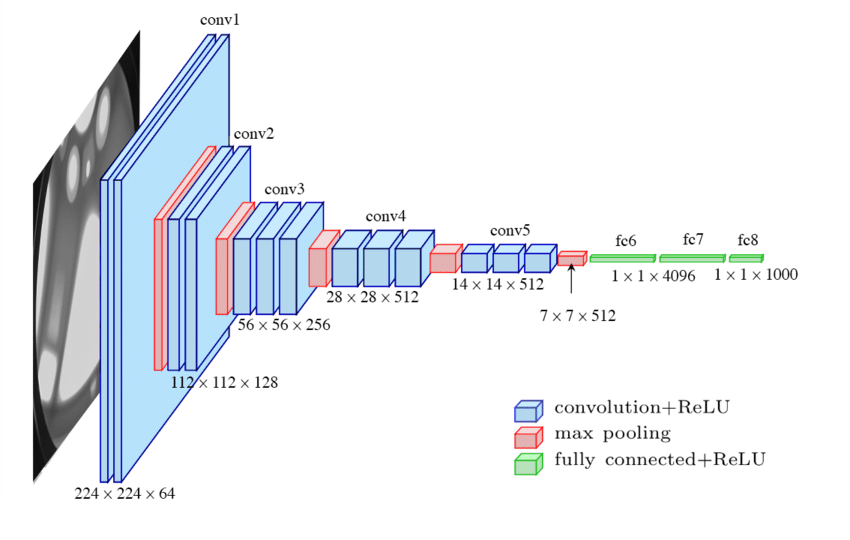
\includegraphics[width=0.85\linewidth,keepaspectratio]{figures/vgg_architecture.png}\\
        {\scriptsize\textcolor{gray}{Credit: Simonyan \& Zisserman (2015), ilustrasi via Medium}}

        \vspace{0.2cm}
        Tiap blok: max-pool $2\times2$ (resolusi $\div 2$), kanal $\times 2$ hingga 512 --- \textbf{spasial mengecil, kanal membesar}.

        \column{0.40\textwidth}
        \centering
        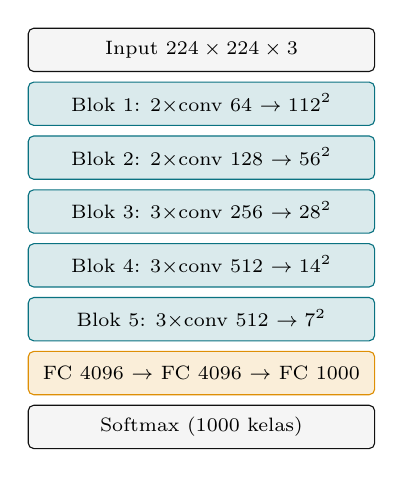
\begin{tikzpicture}[node distance=0.12cm, every node/.style={minimum width=4.4cm}]
            \node[lyr] (in) {Input $224\times224\times3$};
            \node[lyrT, below=of in] (b1) {Blok 1: $2\times$conv 64 $\to 112^2$};
            \node[lyrT, below=of b1] (b2) {Blok 2: $2\times$conv 128 $\to 56^2$};
            \node[lyrT, below=of b2] (b3) {Blok 3: $3\times$conv 256 $\to 28^2$};
            \node[lyrT, below=of b3] (b4) {Blok 4: $3\times$conv 512 $\to 14^2$};
            \node[lyrT, below=of b4] (b5) {Blok 5: $3\times$conv 512 $\to 7^2$};
            \node[lyrO, below=of b5] (fc) {FC 4096 $\to$ FC 4096 $\to$ FC 1000};
            \node[lyr, below=of fc] (sm) {Softmax (1000 kelas)};
        \end{tikzpicture}\\[2pt]
        {\scriptsize\color{dlMute} Resolusi ditulis setelah max-pool tiap blok.}
    \end{columns}
\end{frame}

%------------------------------------------------
\begin{frame}
    \frametitle{Di Mana 138 Juta Parameter VGG-16?}
    \framesubtitle{Analisis Distribusi Bobot}
    \footnotesize

    \begin{columns}[T]
        \column{0.48\textwidth}
        \begin{exampleblock}{Contoh: FC6 (flatten $7\times7\times512$ ke 4096)}
            $$7\cdot7\cdot512\cdot4096 = \mathbf{102{,}8\text{ juta bobot}}$$
        \end{exampleblock}
        \begin{itemize}
            \item Seluruh 13 layer konvolusi: \textbf{14,7 juta} (10,6\%)
            \item 3 layer FC: \textbf{123,6 juta} (89,4\%)
            \item Namun komputasi terbesar ada di conv: \textbf{15,5 GFLOPs} per citra.
        \end{itemize}

        \column{0.48\textwidth}
        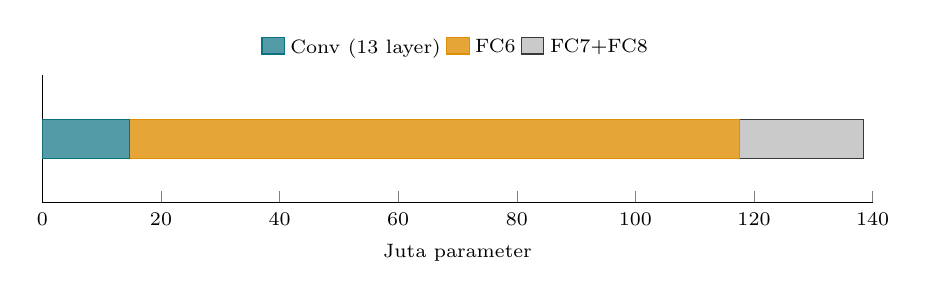
\begin{tikzpicture}
        \begin{axis}[
            xbar stacked, width=\linewidth, height=3.2cm, bar width=14pt,
            xmin=0, xmax=140, xlabel={Juta parameter}, xlabel style={font=\scriptsize},
            ytick=\empty, axis lines*=left, xticklabel style={font=\scriptsize},
            legend style={font=\scriptsize, at={(0.5,1.05)}, anchor=south, legend columns=3, draw=none},
        ]
            \addplot[fill=dlTeal!70, draw=dlTeal] coordinates {(14.7,0)};
            \addplot[fill=dlOrange!80, draw=dlOrange] coordinates {(102.8,0)};
            \addplot[fill=dlHairline, draw=dlCharcoal] coordinates {(20.9,0)};
            \legend{Conv (13 layer), FC6, FC7+FC8}
        \end{axis}
        \end{tikzpicture}

        \begin{alertblock}{Keterbatasan VGG}
            Bobot $>$500 MB, lambat di inferensi. Dorongan berikutnya: \textbf{buang FC raksasa} (GoogLeNet: Global Average Pooling).
        \end{alertblock}
    \end{columns}
\end{frame}

%------------------------------------------------
\begin{frame}[fragile]
    \frametitle{Blok VGG di PyTorch}
    \framesubtitle{Modularitas dalam 8 Baris}
    \footnotesize

    \begin{columns}[T]
        \column{0.60\textwidth}
\begin{lstlisting}[style=py]
def vgg_block(c_in, c_out, n_conv):
    layers = []
    for i in range(n_conv):
        c = c_in if i == 0 else c_out
        layers += [nn.Conv2d(c, c_out, 3, padding=1),
                   nn.ReLU(inplace=True)]
    layers.append(nn.MaxPool2d(2, 2))       # resolusi / 2
    return nn.Sequential(*layers)

# VGG-16: (jumlah conv, kanal) per blok
cfg = [(2, 64), (2, 128), (3, 256), (3, 512), (3, 512)]
\end{lstlisting}

        \column{0.36\textwidth}
        \begin{itemize}
            \item \texttt{padding=1} + $3\times3$ = \textit{same conv}: resolusi hanya berubah di pooling.
            \item VGG-19 cukup mengubah jumlah conv per blok menjadi (2, 2, 4, 4, 4).
            \item Varian \texttt{vgg16\_bn} menyisipkan BatchNorm $\Rightarrow$ top-1 naik 71,6\% $\to$ 73,4\%.
        \end{itemize}
    \end{columns}
\end{frame}

%------------------------------------------------
\begin{frame}
    \frametitle{GoogLeNet (2014): Konvolusi $1\times1$}
    \framesubtitle{Lebih Lebar, Bukan Sekadar Lebih Dalam}
    \footnotesize

    \begin{block}{Ide: $1\times1$ conv sebagai reduksi kanal (\textit{bottleneck})}
        Konvolusi $1\times1$ adalah FC layer per piksel: mencampur kanal tanpa mengubah resolusi.
    \end{block}

    \textbf{Contoh:} input $28\times28\times192$ $\to$ 32 filter $5\times5$ (jumlah perkalian):
    \begin{columns}[T]
        \column{0.48\textwidth}
        \textbf{Langsung:}
        $$28\cdot28\cdot32\cdot(5\cdot5\cdot192) \approx \mathbf{120{,}4\text{ juta}}$$

        \column{0.48\textwidth}
        \textbf{Via $1\times1$ ke 16 kanal dulu:}
        $$\underbrace{28^2\cdot16\cdot192}_{2{,}4\text{ jt}} + \underbrace{28^2\cdot32\cdot(25\cdot16)}_{10{,}0\text{ jt}} \approx \mathbf{12{,}4\text{ juta}}$$
    \end{columns}

    \vspace{0.2cm}
    \begin{itemize}
        \item Hemat \textbf{$\sim$10$\times$} komputasi --- teknik ini dipakai ulang di ResNet bottleneck, MobileNet, dan ConvNeXt.
    \end{itemize}
\end{frame}

%------------------------------------------------
\begin{frame}
    \frametitle{Modul Inception}
    \framesubtitle{Multi-skala dalam Satu Blok}
    \footnotesize

    \begin{columns}[T]
        \column{0.55\textwidth}
        \begin{center}
        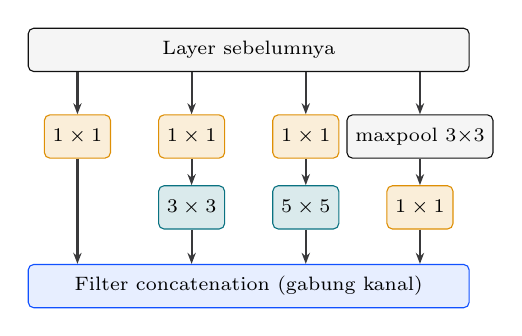
\begin{tikzpicture}[x=1.45cm, y=1cm]
            \node[lyr, minimum width=5.6cm] (in) at (1.5,3) {Layer sebelumnya};
            \node[lyrO] (a1) at (0,1.9) {$1\times1$};
            \node[lyrO] (a2) at (1,1.9) {$1\times1$};
            \node[lyrO] (a3) at (2,1.9) {$1\times1$};
            \node[lyr]  (a4) at (3,1.9) {maxpool $3{\times}3$};
            \node[lyrT] (b2) at (1,1.0) {$3\times3$};
            \node[lyrT] (b3) at (2,1.0) {$5\times5$};
            \node[lyrO] (b4) at (3,1.0) {$1\times1$};
            \node[lyrB, minimum width=5.6cm] (cat) at (1.5,0) {Filter concatenation (gabung kanal)};
            \foreach \n in {a1,a2,a3,a4} \draw[arr] (in.south -| \n.north) -- (\n.north);
            \draw[arr] (a2) -- (b2); \draw[arr] (a3) -- (b3); \draw[arr] (a4) -- (b4);
            \draw[arr] (a1.south) -- (a1.south |- cat.north);
            \foreach \n in {b2,b3,b4} \draw[arr] (\n.south) -- (\n.south |- cat.north);
        \end{tikzpicture}
        \end{center}
        {\scriptsize\color{dlMute} Oranye: $1\times1$ reduksi kanal · Teal: filter spasial $3\times3$ / $5\times5$}

        \column{0.41\textwidth}
        \begin{itemize}
            \item 4 cabang paralel: objek bisa kecil ($1\times1$, $3\times3$) atau besar ($5\times5$) --- \textbf{biarkan jaringan memilih}.
            \item GoogLeNet: 22 layer, 9 modul Inception, juara ILSVRC 2014 (top-5 \textbf{6,7\%}).
            \item Mengganti FC raksasa dengan \textbf{Global Average Pooling}: hanya \textbf{$\sim$6,6 juta} parameter (vs 138 juta VGG-16).
        \end{itemize}
    \end{columns}
\end{frame}

%================================================
\section{Lebih Dalam dengan Residual: ResNet}
\bagian{BAGIAN 02 · RESIDUAL}{ResNet \& Kawan-kawan}{BatchNorm, Degradation Problem, Skip Connection, DenseNet}

%------------------------------------------------
\begin{frame}
    \frametitle{Recap: Batch Normalization}
    \framesubtitle{Prasyarat Melatih Jaringan Dalam (P2)}
    \footnotesize

    \begin{columns}[T]
        \column{0.48\textwidth}
        \begin{block}{Untuk setiap kanal pada mini-batch $B$}
            $$\hat{x}=\frac{x-\mu_B}{\sqrt{\sigma_B^2+\epsilon}}, \qquad y=\gamma\,\hat{x}+\beta$$
        \end{block}
        \begin{itemize}
            \item $\gamma,\beta$ dipelajari; saat \texttt{eval()} memakai \textit{running mean/var}.
            \item Menstabilkan distribusi aktivasi $\Rightarrow$ learning rate lebih besar, tidak sensitif inisialisasi.
        \end{itemize}

        \column{0.48\textwidth}
        \textbf{Pola baku CNN modern:}
        \begin{center}
        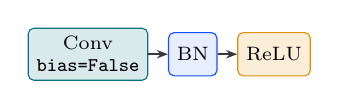
\begin{tikzpicture}[node distance=0.25cm]
            \node[lyrT] (c) {Conv\\\texttt{bias=False}};
            \node[lyrB, right=of c] (b) {BN};
            \node[lyrO, right=of b] (r) {ReLU};
            \draw[arr] (c) -- (b); \draw[arr] (b) -- (r);
        \end{tikzpicture}
        \end{center}
        \begin{itemize}
            \item Bias conv redundan karena $\beta$ BN sudah menggeser.
            \item Tanpa BN, VGG harus dilatih bertahap (11 $\to$ 16 layer); dengan BN, ResNet-152 bisa dilatih langsung.
        \end{itemize}
    \end{columns}
\end{frame}

%------------------------------------------------
\begin{frame}
    \frametitle{Degradation Problem}
    \framesubtitle{Mengapa Tidak Sekadar Menumpuk Layer?}
    \footnotesize

    \begin{columns}[T]
        \column{0.52\textwidth}
        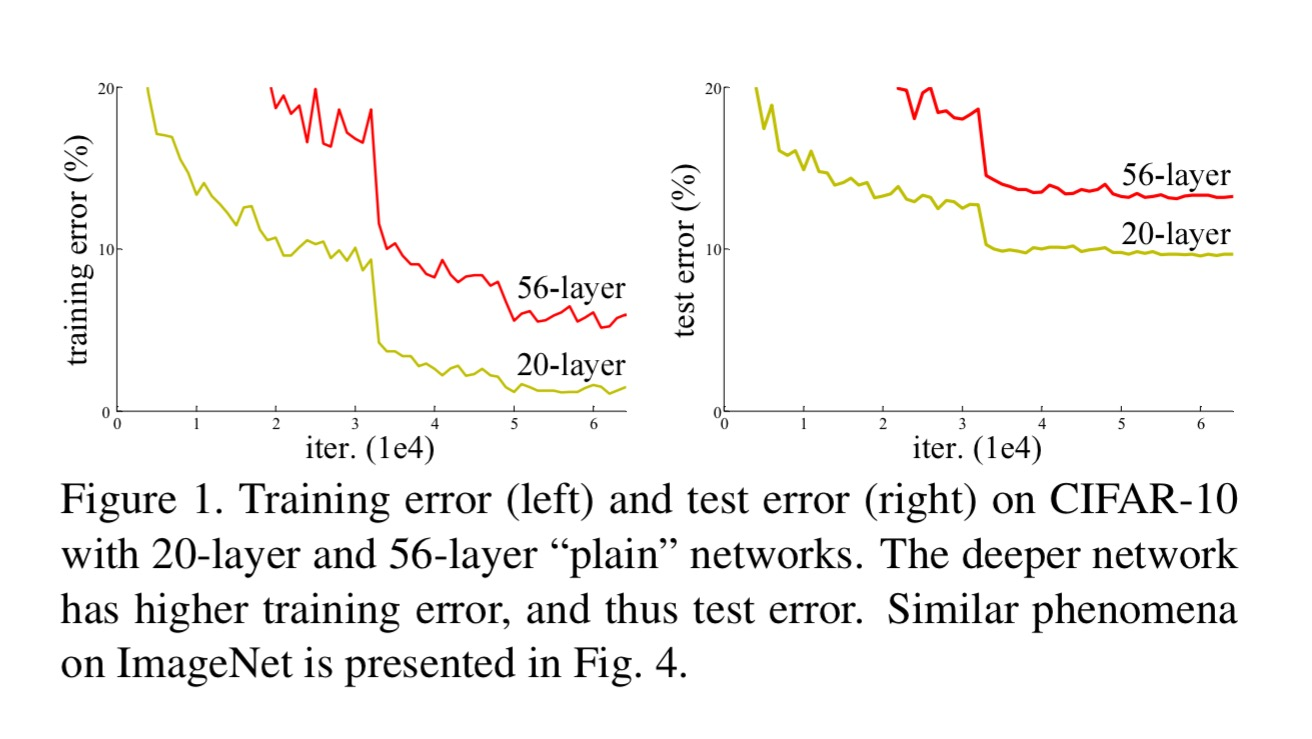
\includegraphics[width=\linewidth]{figures/6_degradation_problems.jpg}\\
        {\scriptsize\textcolor{gray}{Credit: He et al. (2016), CIFAR-10 plain network 20 vs 56 layer}}

        \column{0.44\textwidth}
        \begin{alertblock}{Pengamatan He et al. (2016)}
            Jaringan \textit{plain} 56 layer memiliki \textbf{training error} lebih tinggi daripada 20 layer.
        \end{alertblock}
        \begin{itemize}
            \item \textbf{Bukan overfitting} --- error latih juga naik.
            \item Secara teori, model dalam minimal bisa menyamai model dangkal (layer tambahan $=$ identitas). Namun optimizer \textbf{sulit mempelajari identitas}.
        \end{itemize}
        \vspace{0.1cm}
        \scriptsize
        \begin{tabular}{lcc}
            \toprule
            \textbf{ImageNet top-1 err.} & \textbf{18 layer} & \textbf{34 layer} \\
            \midrule
            Plain & 27,94\% & \con{28,54\%} \\
            ResNet & 27,88\% & \textbf{25,03\%} \\
            \bottomrule
        \end{tabular}
    \end{columns}
\end{frame}

%------------------------------------------------
\begin{frame}
    \frametitle{Residual Learning}
    \framesubtitle{Pelajari Selisihnya, Bukan Pemetaan Utuh}
    \footnotesize

    \begin{columns}[T]
        \column{0.44\textwidth}
        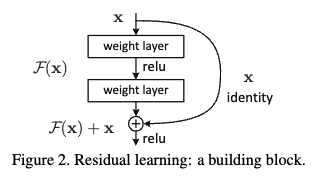
\includegraphics[width=\linewidth]{figures/6_residual_learning.png}\\
        {\scriptsize\textcolor{gray}{Credit: He et al. (2016)}}

        \vspace{0.2cm}
        Bila pemetaan optimal mendekati identitas, cukup dorong $F(x)\to 0$ --- jauh lebih mudah daripada mempelajari $H(x)=x$ dari nol.

        \column{0.52\textwidth}
        \begin{exampleblock}{Formulasi Residual}
            $$H(x) = F(x) + x \quad\Longrightarrow\quad F(x) = H(x) - x$$
        \end{exampleblock}
        \textbf{Aliran gradien (``jalan tol''):}
        $$\frac{\partial L}{\partial x}=\frac{\partial L}{\partial y}\left(1+\frac{\partial F}{\partial x}\right)$$
        \begin{itemize}
            \item Suku \textbf{$+1$}: gradien selalu punya jalur langsung ke layer awal, tidak hilang walau $\partial F/\partial x$ kecil.
            \item Tanpa parameter tambahan dan hampir tanpa komputasi tambahan (hanya penjumlahan).
        \end{itemize}
    \end{columns}
\end{frame}

%------------------------------------------------
\begin{frame}
    \frametitle{Anatomi Basic Block}
    \framesubtitle{Blok Penyusun ResNet-18/34}
    \footnotesize

    \begin{center}
    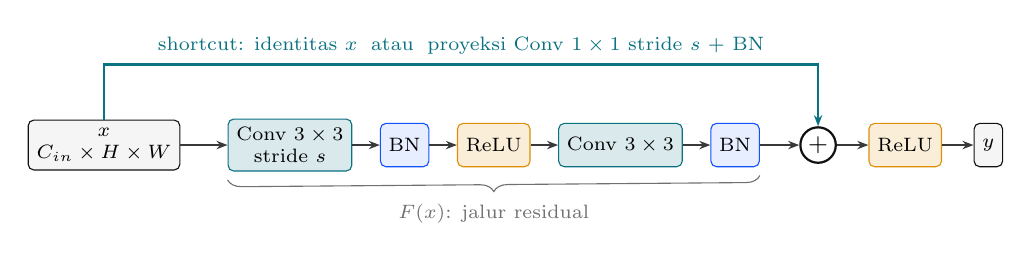
\begin{tikzpicture}[node distance=0.35cm]
        \node[lyr] (x) {$x$\\$C_{in}\times H\times W$};
        \node[lyrT, right=0.6cm of x] (c1) {Conv $3\times3$\\stride $s$};
        \node[lyrB, right=of c1] (b1) {BN};
        \node[lyrO, right=of b1] (r1) {ReLU};
        \node[lyrT, right=of r1] (c2) {Conv $3\times3$};
        \node[lyrB, right=of c2] (b2) {BN};
        \node[addn, right=0.5cm of b2] (add) {$+$};
        \node[lyrO, right=0.4cm of add] (r2) {ReLU};
        \node[lyr, right=0.4cm of r2] (y) {$y$};
        \draw[arr] (x) -- (c1); \draw[arr] (c1) -- (b1); \draw[arr] (b1) -- (r1);
        \draw[arr] (r1) -- (c2); \draw[arr] (c2) -- (b2); \draw[arr] (b2) -- (add);
        \draw[arr] (add) -- (r2); \draw[arr] (r2) -- (y);
        \draw[arr, dlTeal] (x.north) -- ++(0,0.7) -| node[pos=0.25, above, font=\scriptsize, text=dlTeal] {shortcut: identitas $x$ \;atau\; proyeksi Conv $1\times1$ stride $s$ + BN} (add.north);
        \draw[decorate, decoration={brace, mirror, amplitude=5pt}, dlMute] ([yshift=-3pt]c1.south west) -- ([yshift=-3pt]b2.south east) node[midway, below=6pt, font=\scriptsize, text=dlMute] {$F(x)$: jalur residual};
    \end{tikzpicture}
    \end{center}

    \vspace{0.1cm}
    \begin{columns}[T]
        \column{0.48\textwidth}
        \textbf{Identity shortcut} ($s=1$, $C_{in}=C_{out}$)
        \begin{itemize}
            \item $y = \mathrm{ReLU}(F(x) + x)$, nol parameter tambahan.
        \end{itemize}
        \column{0.48\textwidth}
        \textbf{Projection shortcut} (awal tiap stage)
        \begin{itemize}
            \item Resolusi $\div2$ \& kanal $\times2$: $x$ disesuaikan dengan Conv $1\times1$, stride 2.
        \end{itemize}
    \end{columns}
\end{frame}

%------------------------------------------------
\begin{frame}[fragile]
    \frametitle{Basic Block di PyTorch}
    \framesubtitle{Satu Baris yang Mengubah Segalanya}
    \footnotesize

    \begin{columns}[T]
        \column{0.66\textwidth}
\begin{lstlisting}[style=py]
class BasicBlock(nn.Module):
    def __init__(self, c_in, c_out, stride=1):
        super().__init__()
        self.conv1 = nn.Conv2d(c_in, c_out, 3, stride, 1, bias=False)
        self.bn1 = nn.BatchNorm2d(c_out)
        self.conv2 = nn.Conv2d(c_out, c_out, 3, 1, 1, bias=False)
        self.bn2 = nn.BatchNorm2d(c_out)
        self.shortcut = nn.Identity()
        if stride != 1 or c_in != c_out:   # proyeksi
            self.shortcut = nn.Sequential(
                nn.Conv2d(c_in, c_out, 1, stride, bias=False),
                nn.BatchNorm2d(c_out))

    def forward(self, x):
        out = F.relu(self.bn1(self.conv1(x)))
        out = self.bn2(self.conv2(out))
        return F.relu(out + self.shortcut(x))  # <-- skip
\end{lstlisting}

        \column{0.30\textwidth}
        \begin{itemize}
            \item Hapus \texttt{+ self.shortcut(x)} $\Rightarrow$ kembali menjadi \textbf{plain network}.
            \item Eksperimen semester lalu: \textit{Plain-34 $\to$ ResNet-34} hanya dengan menambahkan penjumlahan ini.
            \item Uji: \texttt{BasicBlock(64,128,2)} mengubah $56^2{\times}64 \to 28^2{\times}128$.
        \end{itemize}
    \end{columns}
\end{frame}

%------------------------------------------------
\begin{frame}
    \frametitle{Bottleneck Block (ResNet-50/101/152)}
    \framesubtitle{Reduksi $1\times1$ ala GoogLeNet}
    \footnotesize

    \begin{columns}[T]
        \column{0.44\textwidth}
        \begin{center}
        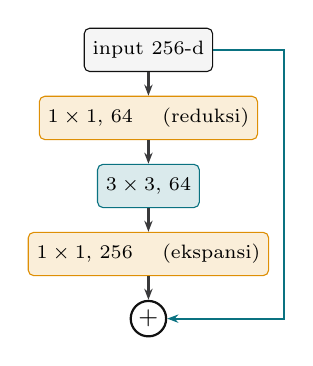
\begin{tikzpicture}[node distance=0.3cm]
            \node[lyr] (x) {input 256-d};
            \node[lyrO, below=of x] (a) {$1\times1$, 64 \quad(reduksi)};
            \node[lyrT, below=of a] (b) {$3\times3$, 64};
            \node[lyrO, below=of b] (c) {$1\times1$, 256 \quad(ekspansi)};
            \node[addn, below=of c] (add) {$+$};
            \draw[arr] (x) -- (a); \draw[arr] (a) -- (b); \draw[arr] (b) -- (c); \draw[arr] (c) -- (add);
            \draw[arr, dlTeal] (x.east) -- ++(0.9,0) |- (add.east);
        \end{tikzpicture}
        \end{center}
        {\scriptsize\color{dlMute} Pola \textbf{lebar $\to$ sempit $\to$ lebar}; BN + ReLU setelah tiap conv (tidak digambar).}

        \column{0.52\textwidth}
        \begin{exampleblock}{Contoh: bobot satu blok pada 256 kanal}
            Basic: $2\cdot(3\cdot3\cdot256\cdot256) = 1.179.648$\\[2pt]
            Bottleneck: $16.384 + 36.864 + 16.384 = \mathbf{69.632}$
        \end{exampleblock}
        \begin{itemize}
            \item $\sim$17$\times$ lebih hemat $\Rightarrow$ blok bisa ditumpuk jauh lebih banyak.
            \item ResNet-50 (bottleneck) vs ResNet-34 (basic): 25,6 vs 21,8 juta parameter, tetapi top-1 \textbf{76,1\%} vs 73,3\%.
        \end{itemize}
    \end{columns}
\end{frame}

%------------------------------------------------
\begin{frame}
    \frametitle{Konfigurasi ResNet-18/34/50}
    \framesubtitle{Empat Stage, Resolusi $\div2$ per Stage}
    \scriptsize
    \vspace{4pt}
    \begin{center}
    \begin{tabular}{llccc}
        \toprule
        \textbf{Stage} & \textbf{Output} & \textbf{ResNet-18} & \textbf{ResNet-34} & \textbf{ResNet-50} \\
        \midrule
        conv1 & $112\times112$ & \multicolumn{3}{c}{$7\times7$, 64, stride 2 \quad+\quad maxpool $3\times3$, stride 2} \\
        conv2\_x & $56\times56$ & $[3\times3, 64]\times2$ & $[3\times3, 64]\times3$ & $[1{\times}1,64 \mid 3{\times}3,64 \mid 1{\times}1,256]\times3$ \\
        conv3\_x & $28\times28$ & $[3\times3, 128]\times2$ & $[3\times3, 128]\times4$ & $[1{\times}1,128 \mid 3{\times}3,128 \mid 1{\times}1,512]\times4$ \\
        conv4\_x & $14\times14$ & $[3\times3, 256]\times2$ & $[3\times3, 256]\times6$ & $[1{\times}1,256 \mid 3{\times}3,256 \mid 1{\times}1,1024]\times6$ \\
        conv5\_x & $7\times7$ & $[3\times3, 512]\times2$ & $[3\times3, 512]\times3$ & $[1{\times}1,512 \mid 3{\times}3,512 \mid 1{\times}1,2048]\times3$ \\
        head & $1\times1$ & \multicolumn{3}{c}{Global Average Pooling \quad+\quad FC 1000} \\
        \midrule
        \multicolumn{2}{l}{\textbf{Parameter / GFLOPs}} & 11,7 jt / 1,8 & 21,8 jt / 3,7 & 25,6 jt / 4,1 \\
        \multicolumn{2}{l}{\textbf{ImageNet top-1}} & 69,8\% & 73,3\% & \textbf{76,1\%} \\
        \bottomrule
    \end{tabular}
    \end{center}
    \vspace{0.15cm}
    \footnotesize
    \begin{itemize}
        \item Downsampling memakai \textbf{conv stride 2} di awal stage (bukan pooling), lalu \textbf{GAP} menggantikan FC raksasa VGG.
        \item ResNet-101/152: pola bottleneck yang sama, conv4\_x diulang 23/36 kali.
    \end{itemize}
\end{frame}

%------------------------------------------------
\begin{frame}
    \frametitle{DenseNet (2017): Gabungkan, Jangan Jumlahkan}
    \framesubtitle{Dense Connectivity}
    \footnotesize

    \begin{columns}[T]
        \column{0.48\textwidth}
        \begin{center}
        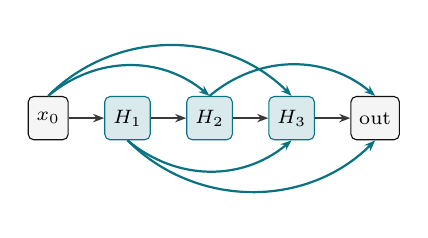
\begin{tikzpicture}[node distance=0.45cm]
            \node[lyr] (x0) {$x_0$};
            \node[lyrT, right=of x0] (h1) {$H_1$};
            \node[lyrT, right=of h1] (h2) {$H_2$};
            \node[lyrT, right=of h2] (h3) {$H_3$};
            \node[lyr, right=of h3] (o) {out};
            \draw[arr] (x0) -- (h1); \draw[arr] (h1) -- (h2); \draw[arr] (h2) -- (h3); \draw[arr] (h3) -- (o);
            \draw[arr, dlTeal] (x0.north) to[bend left=40] (h2.north);
            \draw[arr, dlTeal] (x0.north) to[bend left=45] (h3.north);
            \draw[arr, dlTeal] (h1.south) to[bend right=40] (h3.south);
            \draw[arr, dlTeal] (h1.south) to[bend right=45] (o.south);
            \draw[arr, dlTeal] (h2.north) to[bend left=40] (o.north);
        \end{tikzpicture}
        \end{center}
        \vspace{0.2cm}
        \begin{center}
        \setlength{\tabcolsep}{4pt}
        \begin{tabular}{lcc}
            \toprule
             & \textbf{ResNet} & \textbf{DenseNet} \\
            \midrule
            Operasi & $x + F(x)$ & $[x_0,\dots,x_{\ell-1}]$ (concat) \\
            Params & 25,6 jt (R-50) & \textbf{8,0 jt} (D-121) \\
            Top-1 & 76,1\% & 74,4\% \\
            \bottomrule
        \end{tabular}
        \end{center}

        \column{0.48\textwidth}
        \begin{block}{Setiap layer menerima semua fitur sebelumnya}
            $$x_\ell = H_\ell\big([x_0, x_1, \dots, x_{\ell-1}]\big)$$
        \end{block}
        \begin{itemize}
            \item \textbf{Growth rate} $k$ (mis. 32): tiap layer hanya menambah $k$ kanal baru $\Rightarrow$ layer sempit, fitur dipakai ulang.
            \item \textbf{Transition layer} ($1\times1$ conv + avgpool $2\times2$) mengontrol ledakan kanal antar blok.
            \item Hemat parameter, namun boros memori aktivasi saat training.
        \end{itemize}
    \end{columns}
\end{frame}

%================================================
\section{CNN Efisien: MobileNet \& EfficientNet}
\bagian{BAGIAN 03 · EFISIENSI}{MobileNet \& EfficientNet}{Depthwise Separable Convolution, Inverted Residual, Compound Scaling}

%------------------------------------------------
\begin{frame}
    \frametitle{Standar vs Depthwise Separable}
    \framesubtitle{Memecah Satu Konvolusi Menjadi Dua}
    \footnotesize

    \textbf{Motivasi:} ponsel, drone, kamera IoT --- latensi \& energi terbatas. ResNet-50 butuh 4,1 GFLOPs per citra.

    \vspace{0.1cm}
    Notasi: kernel $D_K\times D_K$, kanal masuk $M$, kanal keluar $N$, feature map $D_F\times D_F$.
    \begin{columns}[T]
        \column{0.48\textwidth}
        \begin{block}{Konvolusi standar}
            $$D_K^2 \cdot M \cdot N \cdot D_F^2$$
            Filter spasial \textbf{dan} pencampuran kanal sekaligus.
        \end{block}

        \column{0.48\textwidth}
        \begin{exampleblock}{Depthwise + Pointwise}
            $$\underbrace{D_K^2 \cdot M \cdot D_F^2}_{\text{depthwise}} + \underbrace{M \cdot N \cdot D_F^2}_{\text{pointwise } 1\times1}$$
            Filter spasial per kanal, lalu campur kanal.
        \end{exampleblock}
    \end{columns}
    \vspace{0.2cm}
    \textbf{Rasio biaya:}
    $$\frac{\text{separable}}{\text{standar}} = \frac{1}{N} + \frac{1}{D_K^2} \quad\Rightarrow\quad \text{untuk } 3\times3 \text{ dan } N \text{ besar: } \approx \tfrac{1}{9} \;(\text{hemat } 8\text{--}9\times)$$
\end{frame}

%------------------------------------------------
\begin{frame}
    \frametitle{Contoh Numerik \& Visualisasi}
    \framesubtitle{$3\times3$, $M=N=256$, $D_F=56$}
    \footnotesize

    \begin{columns}[T]
        \column{0.46\textwidth}
        \vspace{4pt}
        \begin{center}
        \begin{tabular}{lrr}
            \toprule
             & \textbf{Mult-adds} & \textbf{Bobot} \\
            \midrule
            Standar & 1,85 G & 589.824 \\
            Depthwise & 0,007 G & 2.304 \\
            Pointwise & 0,206 G & 65.536 \\
            \midrule
            \textbf{Separable} & \textbf{0,21 G} & \textbf{67.840} \\
            \bottomrule
        \end{tabular}
        \end{center}
        \vspace{0.1cm}
        \begin{itemize}
            \item Hemat \textbf{$8{,}7\times$}, sesuai rumus $\tfrac{1}{256}+\tfrac{1}{9}\approx 0{,}115$.
            \item $\sim$97\% biaya kini ada di pointwise $1\times1$ (operasi matriks yang sangat efisien di hardware).
        \end{itemize}

        \column{0.50\textwidth}
        \begin{center}
        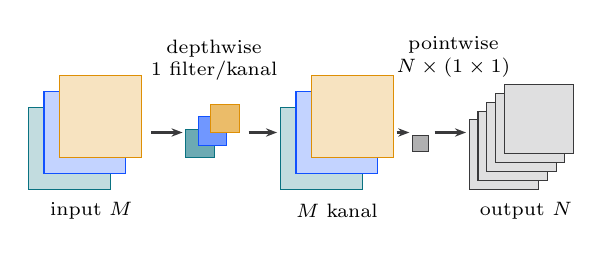
\begin{tikzpicture}[x=0.8cm,y=0.8cm]
            % input channels
            \foreach \i/\c in {0/dlTeal, 1/dlBlue, 2/dlOrange} {
                \fill[\c!25, draw=\c] (0.25*\i,0.25*\i) rectangle ++(1.3,1.3);
            }
            \node[font=\scriptsize] at (1.0,-0.35) {input $M$};
            % depthwise kernels
            \foreach \i/\c in {0/dlTeal, 1/dlBlue, 2/dlOrange} {
                \fill[\c!60, draw=\c] (2.5+0.2*\i,0.5+0.2*\i) rectangle ++(0.45,0.45);
            }
            \node[font=\scriptsize, align=center] at (2.95,2.05) {depthwise\\1 filter/kanal};
            \foreach \i/\c in {0/dlTeal, 1/dlBlue, 2/dlOrange} {
                \fill[\c!25, draw=\c] (4.0+0.25*\i,0.25*\i) rectangle ++(1.3,1.3);
            }
            \node[font=\scriptsize] at (4.9,-0.35) {$M$ kanal};
            % pointwise
            \fill[dlCharcoal!40, draw=dlCharcoal] (6.1,0.6) rectangle ++(0.25,0.25);
            \node[font=\scriptsize, align=center] at (6.75,2.1) {pointwise\\$N\times(1\times1)$};
            \foreach \i in {0,...,4} {
                \fill[dlHairline!60, draw=dlCharcoal] (7.0+0.14*\i,0.14*\i) rectangle ++(1.1,1.1);
            }
            \node[font=\scriptsize] at (7.9,-0.35) {output $N$};
            \draw[arr] (1.95,0.9) -- (2.45,0.9);
            \draw[arr] (3.5,0.9) -- (3.95,0.9);
            \draw[arr] (5.85,0.9) -- (6.05,0.9);
            \draw[arr] (6.45,0.9) -- (6.95,0.9);
        \end{tikzpicture}
        \end{center}
        \vspace{0.3cm}
        {\scriptsize\color{dlMute} Depthwise: tiap kanal difilter sendiri (tanpa mencampur). Pointwise: $N$ filter $1\times1$ mencampur informasi antar kanal.}
    \end{columns}
\end{frame}

%------------------------------------------------
\begin{frame}[fragile]
    \frametitle{MobileNetV1 (2017) di PyTorch}
    \framesubtitle{Kuncinya: Argumen \texttt{groups}}
    \footnotesize

    \begin{columns}[T]
        \column{0.63\textwidth}
\begin{lstlisting}[style=py]
def dw_separable(c_in, c_out, stride=1):
    return nn.Sequential(
        # depthwise: groups=c_in -> 1 filter per kanal
        nn.Conv2d(c_in, c_in, 3, stride, 1,
                  groups=c_in, bias=False),
        nn.BatchNorm2d(c_in), nn.ReLU(inplace=True),
        # pointwise: konvolusi 1x1 mencampur kanal
        nn.Conv2d(c_in, c_out, 1, bias=False),
        nn.BatchNorm2d(c_out), nn.ReLU(inplace=True))
\end{lstlisting}
        {\scriptsize\color{dlMute} Cek: bobot conv \texttt{dw\_separable(256,256)} $=67.840$ vs \texttt{nn.Conv2d(256,256,3)} $=589.824$.}

        \column{0.33\textwidth}
        \textbf{Dua ``kenop'' efisiensi MobileNet:}
        \begin{itemize}
            \item \textbf{Width multiplier} $\alpha\in\{1; 0{,}75; 0{,}5; 0{,}25\}$: kanal $M,N \to \alpha M, \alpha N$.
            \item \textbf{Resolution multiplier} $\rho$: input $224\to192\to160\to128$.
            \item Biaya turun $\approx\alpha^2\rho^2$.
        \end{itemize}
        \vspace{0.1cm}
        MobileNetV1: 4,2 juta parameter, 0,57 G mult-adds, top-1 70,6\% --- mendekati VGG-16 dengan komputasi $\sim$27$\times$ lebih kecil.
    \end{columns}
\end{frame}

%------------------------------------------------
\begin{frame}
    \frametitle{MobileNetV2 (2018): Inverted Residual}
    \framesubtitle{Sempit $\to$ Lebar $\to$ Sempit}
    \footnotesize

    \begin{columns}[T]
        \column{0.38\textwidth}
        \begin{center}
        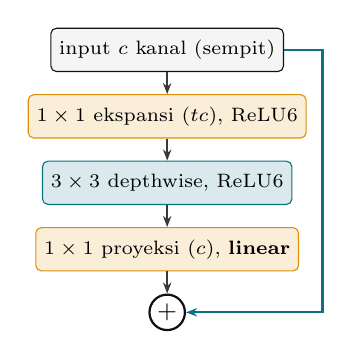
\begin{tikzpicture}[node distance=0.28cm]
            \node[lyr] (x) {input $c$ kanal (sempit)};
            \node[lyrO, below=of x] (a) {$1\times1$ ekspansi ($tc$), ReLU6};
            \node[lyrT, below=of a] (b) {$3\times3$ depthwise, ReLU6};
            \node[lyrO, below=of b] (c) {$1\times1$ proyeksi ($c$), \textbf{linear}};
            \node[addn, below=of c] (add) {$+$};
            \draw[arr] (x) -- (a); \draw[arr] (a) -- (b); \draw[arr] (b) -- (c); \draw[arr] (c) -- (add);
            \draw[arr, dlTeal] (x.east) -- ([xshift=0.2cm]x.east -| a.east) |- (add.east);
        \end{tikzpicture}
        \end{center}
        {\scriptsize\color{dlMute} Faktor ekspansi $t=6$; skip hanya bila stride 1 \& $c_{in}=c_{out}$.}

        \column{0.58\textwidth}
        \vspace{2pt}
        \begin{center}
        \scriptsize
        \begin{tabular}{lll}
            \toprule
             & \textbf{ResNet bottleneck} & \textbf{MBv2 inverted} \\
            \midrule
            Bentuk & lebar--sempit--lebar & \textbf{sempit--lebar--sempit} \\
            Conv tengah & $3\times3$ standar & $3\times3$ \textbf{depthwise} \\
            Skip antar & tensor lebar & tensor sempit \\
            Aktivasi akhir & ReLU & \textbf{linear} \\
            \bottomrule
        \end{tabular}
        \end{center}
        \begin{itemize}
            \item \textbf{Linear bottleneck:} ReLU pada tensor sempit membuang informasi, maka proyeksi dibiarkan linear.
            \item MobileNetV2: 3,5 juta parameter, 0,30 GFLOPs, top-1 \textbf{71,9\%}. Blok ini menjadi fondasi EfficientNet \& ConvNeXt.
        \end{itemize}
    \end{columns}
\end{frame}

%------------------------------------------------
\begin{frame}
    \frametitle{EfficientNet (2019): Compound Scaling}
    \framesubtitle{Skalakan Tiga Dimensi Sekaligus}
    \footnotesize

    \begin{columns}[T]
        \column{0.48\textwidth}
        \textbf{Masalah:} memperbesar model biasanya hanya satu dimensi --- lebih dalam (ResNet-152), lebih lebar (WideResNet), atau resolusi lebih tinggi. Hasilnya cepat jenuh.
        \begin{exampleblock}{Compound scaling dengan koefisien $\phi$}
            $$d=\alpha^{\phi},\quad w=\beta^{\phi},\quad r=\gamma^{\phi}$$
            $$\text{s.t. } \alpha\cdot\beta^2\cdot\gamma^2\approx 2$$
        \end{exampleblock}
        {\scriptsize FLOPs $\propto d\cdot w^2\cdot r^2$, sehingga tiap $\phi+1$ menggandakan FLOPs. Hasil grid search: $\alpha=1{,}2$, $\beta=1{,}1$, $\gamma=1{,}15$.}

        \column{0.48\textwidth}
        \begin{itemize}
            \item \textbf{Baseline B0}: dicari dengan Neural Architecture Search; blok MBConv (inverted residual MobileNetV2 + Squeeze-and-Excitation).
            \item B0 $\to$ B7: naikkan $\phi$ saja.
        \end{itemize}
        \vspace{4pt}
        \begin{center}
        \begin{tabular}{lrrr}
            \toprule
            \textbf{Model} & \textbf{Params} & \textbf{Input} & \textbf{Top-1} \\
            \midrule
            EfficientNet-B0 & 5,3 jt & 224 & 77,7\% \\
            EfficientNet-B7 & 66 jt & 600 & 84,3\% \\
            ResNet-50 & 25,6 jt & 224 & 76,1\% \\
            \bottomrule
        \end{tabular}
        \end{center}
        {\scriptsize\color{dlMute} B0 lebih akurat dari ResNet-50 dengan $\sim$5$\times$ lebih sedikit parameter.}
    \end{columns}
\end{frame}

%================================================
\section{ConvNeXt: CNN untuk Era 2020-an}
\bagian{BAGIAN 04 · CNN MODERN}{ConvNeXt}{``A ConvNet for the 2020s'': Memodernisasi ResNet dengan Resep Transformer}

%------------------------------------------------
\begin{frame}
    \frametitle{Konteks: CNN vs Vision Transformer}
    \framesubtitle{Apakah Keunggulan ViT dari Attention?}
    \footnotesize

    \begin{columns}[T]
        \column{0.48\textwidth}
        \begin{alertblock}{2020--2021: Transformer masuk ke Vision}
            ViT (2020) dan Swin Transformer (2021) melampaui ResNet di ImageNet; muncul narasi ``CNN akan tergantikan''.
        \end{alertblock}
        \begin{itemize}
            \item Namun Swin juga memakai \textbf{jendela lokal} dan \textbf{hierarki stage} --- mirip CNN.
            \item Selain arsitektur, Transformer datang dengan \textbf{resep training baru}: AdamW, 300 epoch, Mixup/CutMix, RandAugment, label smoothing, stochastic depth.
        \end{itemize}

        \column{0.48\textwidth}
        \begin{exampleblock}{Pertanyaan Liu et al. (Meta AI, 2022)}
            Bila ResNet-50 dimodernisasi \textbf{langkah demi langkah} memakai pilihan desain Transformer, seberapa jauh CNN murni bisa bersaing?
        \end{exampleblock}
        \vspace{2pt}
        \begin{center}
        \begin{tabular}{lrr}
            \toprule
            \textbf{Model} & \textbf{GFLOPs} & \textbf{Top-1} \\
            \midrule
            ResNet-50 (resep lama) & 4,1 & 76,1\% \\
            Swin-T & 4,5 & 81,3\% \\
            \textbf{ConvNeXt-T} & 4,5 & \textbf{82,1\%} \\
            \bottomrule
        \end{tabular}
        \end{center}
    \end{columns}
\end{frame}

%------------------------------------------------
\begin{frame}
    \frametitle{Roadmap: ResNet-50 $\to$ ConvNeXt-T}
    \framesubtitle{Kontribusi Tiap Modifikasi (ImageNet Top-1)}
    \footnotesize

    \begin{columns}[T]
        \column{0.62\textwidth}
        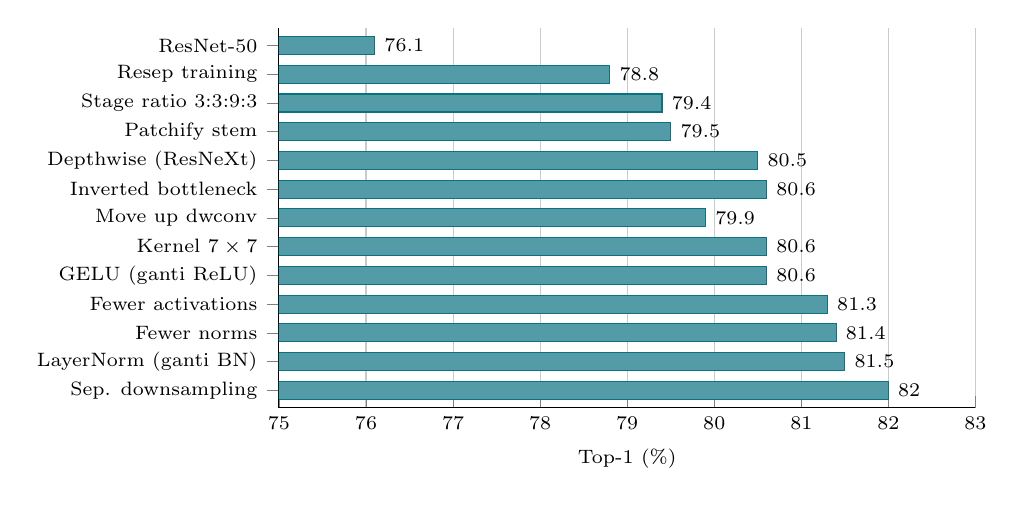
\begin{tikzpicture}
        \begin{axis}[
            xbar, width=0.86\linewidth, height=6.4cm, bar width=6.5pt,
            xmin=75, xmax=83, xlabel={Top-1 (\%)}, xlabel style={font=\scriptsize},
            ytick={0,...,12}, yticklabels={{ResNet-50}, {Resep training}, {Stage ratio 3:3:9:3}, {Patchify stem}, {Depthwise (ResNeXt)}, {Inverted bottleneck}, {Move up dwconv}, {Kernel $7\times7$}, {GELU (ganti ReLU)}, {Fewer activations}, {Fewer norms}, {LayerNorm (ganti BN)}, {Sep. downsampling}},
            yticklabel style={font=\scriptsize}, xticklabel style={font=\scriptsize},
            y dir=reverse, nodes near coords, every node near coord/.append style={font=\scriptsize},
            axis lines*=left, xmajorgrids, grid style={dlHairline}, enlarge y limits=0.05,
        ]
            \addplot[fill=dlTeal!70, draw=dlTeal] coordinates {
                (76.1,0) (78.8,1) (79.4,2) (79.5,3) (80.5,4) (80.6,5) (79.9,6) (80.6,7)
                (80.6,8) (81.3,9) (81.4,10) (81.5,11) (82.0,12)};
        \end{axis}
        \end{tikzpicture}

        \column{0.34\textwidth}
        \begin{itemize}
            \item \textbf{Resep training} saja: +2,7 poin --- sebagian ``keunggulan Transformer'' ternyata dari cara melatihnya.
            \item \textbf{Makro}: stage ratio ala Swin, stem $4\times4$ stride 4 (\textit{patchify}).
            \item \textbf{Blok}: depthwise, inverted bottleneck, kernel $7\times7$.
            \item \textbf{Mikro}: GELU, lebih sedikit aktivasi \& normalisasi, LayerNorm.
        \end{itemize}
        {\scriptsize\color{dlMute} Sumber: Liu et al. (2022), Fig. 2.}
    \end{columns}
\end{frame}

%------------------------------------------------
\begin{frame}
    \frametitle{Blok ResNet vs Blok ConvNeXt}
    \framesubtitle{Elemen yang Diadopsi dari Transformer}
    \footnotesize

    \begin{columns}[T]
        \column{0.30\textwidth}
        \centering\textbf{ResNet bottleneck}\\[4pt]
        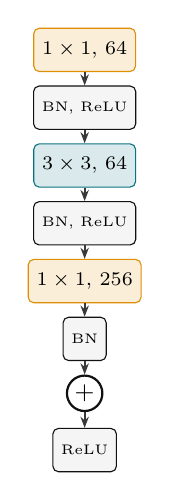
\begin{tikzpicture}[node distance=0.17cm]
            \node[lyrO] (a) {$1\times1$, 64};
            \node[lyr, below=of a, font=\tiny] (a2) {BN, ReLU};
            \node[lyrT, below=of a2] (b) {$3\times3$, 64};
            \node[lyr, below=of b, font=\tiny] (b2) {BN, ReLU};
            \node[lyrO, below=of b2] (c) {$1\times1$, 256};
            \node[lyr, below=of c, font=\tiny] (c2) {BN};
            \node[addn, below=of c2] (add) {$+$};
            \node[lyr, below=0.2cm of add, font=\tiny] (r) {ReLU};
            \foreach \u/\v in {a/a2,a2/b,b/b2,b2/c,c/c2,c2/add,add/r} \draw[arr] (\u) -- (\v);
        \end{tikzpicture}

        \column{0.30\textwidth}
        \centering\textbf{ConvNeXt block}\\[4pt]
        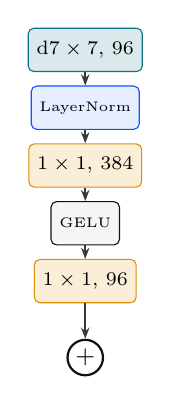
\begin{tikzpicture}[node distance=0.17cm]
            \node[lyrT] (a) {d$7\times7$, 96};
            \node[lyrB, below=of a, font=\tiny] (a2) {LayerNorm};
            \node[lyrO, below=of a2] (b) {$1\times1$, 384};
            \node[lyr, below=of b, font=\tiny] (b2) {GELU};
            \node[lyrO, below=of b2] (c) {$1\times1$, 96};
            \node[addn, below=0.45cm of c] (add) {$+$};
            \foreach \u/\v in {a/a2,a2/b,b/b2,b2/c,c/add} \draw[arr] (\u) -- (\v);
        \end{tikzpicture}

        \column{0.36\textwidth}
        \textbf{Padanan dengan Transformer:}
        \begin{itemize}
            \item \textbf{Patchify stem} $4\times4$/4 $\leftrightarrow$ patch embedding ViT.
            \item \textbf{Depthwise $7\times7$} $\leftrightarrow$ pencampuran spasial per kanal (seperti self-attention per jendela Swin).
            \item \textbf{$1\times1$ ekspansi $4\times$} $\leftrightarrow$ MLP/FFN $4\times$.
            \item \textbf{1 GELU + 1 LN} per blok, seperti blok Transformer.
            \item Downsampling terpisah (LN + conv $2\times2$/2) di antara stage.
        \end{itemize}
    \end{columns}
\end{frame}

%------------------------------------------------
\begin{frame}[fragile]
    \frametitle{ConvNeXt Block di PyTorch}
    \framesubtitle{Versi Ringkas (tanpa Layer Scale)}
    \footnotesize

    \begin{columns}[T]
        \column{0.64\textwidth}
\begin{lstlisting}[style=py]
class ConvNeXtBlock(nn.Module):
    def __init__(self, dim):
        super().__init__()
        self.dwconv = nn.Conv2d(dim, dim, 7, padding=3, groups=dim)
        self.norm = nn.LayerNorm(dim)      # channels-last
        self.pw1 = nn.Linear(dim, 4 * dim) # 1x1, ekspansi 4x
        self.act = nn.GELU()
        self.pw2 = nn.Linear(4 * dim, dim) # 1x1, proyeksi

    def forward(self, x):                  # (B, C, H, W)
        y = self.dwconv(x).permute(0, 2, 3, 1)   # (B, H, W, C)
        y = self.pw2(self.act(self.pw1(self.norm(y))))
        return x + y.permute(0, 3, 1, 2)         # residual
\end{lstlisting}

        \column{0.32\textwidth}
        \begin{itemize}
            \item \texttt{nn.Linear} pada tensor \textit{channels-last} $=$ konvolusi $1\times1$.
            \item Mirip inverted bottleneck MobileNetV2, tetapi depthwise dipindah ke \textbf{awal} blok.
            \item ConvNeXt-T: stage (3, 3, 9, 3), kanal (96, 192, 384, 768), 28,6 juta parameter.
            \item Versi resmi menambah \textit{layer scale} \& \textit{stochastic depth}.
        \end{itemize}
    \end{columns}
\end{frame}

%================================================
\section{Perbandingan Arsitektur}
\bagian{BAGIAN 05 · PERBANDINGAN}{Perbandingan Arsitektur}{Akurasi, Parameter, dan Komputasi pada ImageNet}

%------------------------------------------------
\begin{frame}
    \frametitle{Tabel Perbandingan pada ImageNet-1K}
    \framesubtitle{Bobot Pretrained torchvision}
    \scriptsize
    \vspace{4pt}
    \begin{center}
    \begin{tabular}{llrrrl}
        \toprule
        \textbf{Model} & \textbf{Tahun} & \textbf{Params (jt)} & \textbf{GFLOPs} & \textbf{Top-1 (\%)} & \textbf{Ide kunci} \\
        \midrule
        AlexNet & 2012 & 61,1 & 0,71 & 56,5 & ReLU, dropout, GPU \\
        VGG-16 & 2014 & 138,4 & \con{15,47} & 71,6 & tumpukan $3\times3$ \\
        GoogLeNet & 2014 & 6,6 & 1,50 & 69,8 & Inception, $1\times1$, GAP \\
        ResNet-18 & 2015 & 11,7 & 1,81 & 69,8 & residual (basic block) \\
        ResNet-50 & 2015 & 25,6 & 4,09 & 76,1 & residual (bottleneck) \\
        DenseNet-121 & 2017 & 8,0 & 2,83 & 74,4 & dense concatenation \\
        MobileNetV2 & 2018 & \textbf{3,5} & 0,30 & 71,9 & inverted residual \\
        MobileNetV3-L & 2019 & 5,5 & \textbf{0,22} & 74,0 & NAS + SE + h-swish \\
        EfficientNet-B0 & 2019 & 5,3 & 0,39 & 77,7 & compound scaling \\
        ConvNeXt-T & 2022 & 28,6 & 4,46 & \textbf{82,5} & modernisasi ResNet \\
        \bottomrule
    \end{tabular}
    \end{center}
    \vspace{0.1cm}
    {\scriptsize\color{dlMute} Angka dari dokumentasi \texttt{torchvision.models} (evaluasi single-crop $224\times224$) --- sama dengan bobot yang akan dipakai pada Studio Proyek 2 (Pertemuan 6).}

    \vspace{0.1cm}
    \footnotesize
    \textbf{Observasi:} VGG-16 memakai 40$\times$ parameter dan 70$\times$ komputasi MobileNetV2 untuk akurasi yang hampir sama.
\end{frame}

%------------------------------------------------
\begin{frame}
    \frametitle{Akurasi vs Komputasi}
    \framesubtitle{Frontier Efisiensi Arsitektur CNN}
    \footnotesize

    \begin{columns}[T]
        \column{0.64\textwidth}
        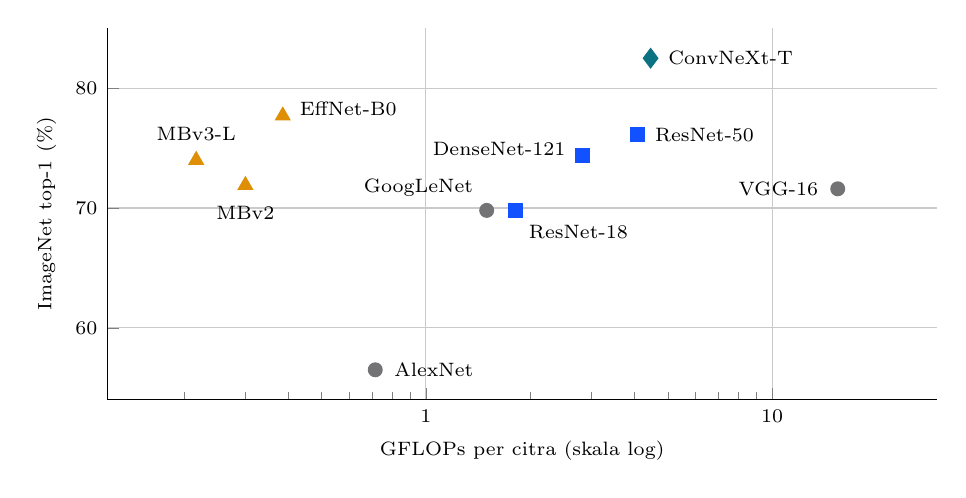
\begin{tikzpicture}
        \begin{axis}[
            width=\linewidth, height=6.3cm, xmode=log,
            xmin=0.12, xmax=30, ymin=54, ymax=85,
            xlabel={GFLOPs per citra (skala log)}, ylabel={ImageNet top-1 (\%)},
            xlabel style={font=\scriptsize}, ylabel style={font=\scriptsize},
            xticklabel style={font=\scriptsize}, yticklabel style={font=\scriptsize},
            log ticks with fixed point, axis lines*=left, grid=major, grid style={dlHairline},
        ]
            \addplot[only marks, mark=*, mark size=2.5pt, color=dlHairline!40!dlCharcoal] coordinates {(0.714,56.5) (15.47,71.6) (1.498,69.8)};
            \addplot[only marks, mark=square*, mark size=2.5pt, color=dlBlue] coordinates {(1.814,69.8) (4.089,76.1) (2.834,74.4)};
            \addplot[only marks, mark=triangle*, mark size=3pt, color=dlOrange] coordinates {(0.301,71.9) (0.217,74.0) (0.386,77.7)};
            \addplot[only marks, mark=diamond*, mark size=3.5pt, color=dlTeal] coordinates {(4.456,82.5)};
            \node[anchor=west, font=\scriptsize] at (axis cs:0.76,56.5) {AlexNet};
            \node[anchor=east, font=\scriptsize] at (axis cs:14.5,71.6) {VGG-16};
            \node[anchor=south east, font=\scriptsize] at (axis cs:1.46,70.2) {GoogLeNet};
            \node[anchor=north west, font=\scriptsize] at (axis cs:1.86,69.4) {ResNet-18};
            \node[anchor=west, font=\scriptsize] at (axis cs:4.3,76.1) {ResNet-50};
            \node[anchor=east, font=\scriptsize] at (axis cs:2.7,74.9) {DenseNet-121};
            \node[anchor=north, font=\scriptsize] at (axis cs:0.301,71.0) {MBv2};
            \node[anchor=south, font=\scriptsize] at (axis cs:0.217,74.8) {MBv3-L};
            \node[anchor=west, font=\scriptsize] at (axis cs:0.405,78.3) {EffNet-B0};
            \node[anchor=west, font=\scriptsize] at (axis cs:4.7,82.5) {ConvNeXt-T};
        \end{axis}
        \end{tikzpicture}

        \column{0.32\textwidth}
        \textbf{Legenda:}
        \begin{itemize}
            \item \textcolor{dlHairline!40!dlCharcoal}{$\bullet$} Klasik (2012--2014)
            \item \textcolor{dlBlue}{$\blacksquare$} Residual / dense
            \item \textcolor{dlOrange}{$\blacktriangle$} Efisien (mobile)
            \item \textcolor{dlTeal}{$\blacklozenge$} Modern (2022)
        \end{itemize}
        \vspace{0.1cm}
        \textbf{Takeaway:} kemajuan arsitektur bukan sekadar ``lebih besar''. Model di kiri atas (EfficientNet, MobileNetV3) mencapai akurasi lebih tinggi dengan komputasi $\sim$40$\times$ lebih kecil daripada VGG.
    \end{columns}
\end{frame}

%------------------------------------------------
\begin{frame}[fragile]
    \frametitle{Memilih Backbone dalam Praktik}
    \framesubtitle{Jembatan ke Studio Proyek 2 (P6)}
    \footnotesize

    \begin{columns}[T]
        \column{0.42\textwidth}
        \vspace{2pt}
        \scriptsize\setlength{\tabcolsep}{3pt}
        \begin{tabular}{ll}
            \toprule
            \textbf{Kebutuhan} & \textbf{Kandidat} \\
            \midrule
            Baseline umum & ResNet-18 / 50 \\
            Edge / mobile & MobileNetV3, EffNet-B0\hspace{-2pt} \\
            Akurasi maksimum & ConvNeXt-T / S \\
            Parameter minim & DenseNet-121 \\
            Pembanding historis & AlexNet, VGG-16 \\
            \bottomrule
        \end{tabular}

        \column{0.54\textwidth}
\begin{lstlisting}[style=py]
from torchvision import models
m = models.resnet50(weights="IMAGENET1K_V1")
m.fc = nn.Linear(m.fc.in_features, 5)
# head lain -> MobileNetV3: m.classifier[3]
#               ConvNeXt   : m.classifier[2]
\end{lstlisting}
        \begin{itemize}
            \item Semua backbone di atas tersedia \textbf{pretrained} di \texttt{torchvision.models}.
            \item Pertemuan 6: bandingkan backbone \& strategi fine-tuning (freezing, linear probing vs full fine-tuning).
        \end{itemize}
    \end{columns}
\end{frame}

%================================================
\section{Dari Klasifikasi ke Deteksi \& Segmentasi}
\bagian{BAGIAN 06 · DETEKSI \& SEGMENTASI}{Beyond Classification}{Format Bounding Box, IoU, mAP, R-CNN, YOLO, FCN, U-Net, Mask R-CNN}

%------------------------------------------------
\begin{frame}
    \frametitle{Empat Tugas Computer Vision}
    \framesubtitle{Dari ``Apa'' Menuju ``Di Mana''}
    \footnotesize

    \begin{center}
    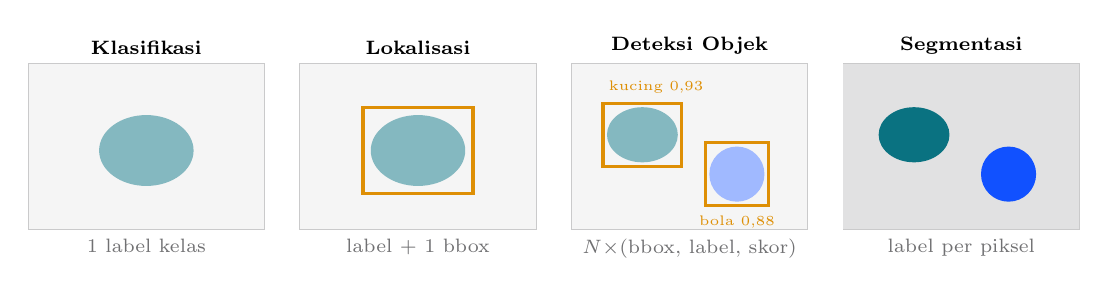
\begin{tikzpicture}[x=1cm,y=1cm]
        \foreach \i/\ttl in {0/Klasifikasi, 1/Lokalisasi, 2/Deteksi Objek, 3/Segmentasi} {
            \begin{scope}[xshift=\i*3.45cm]
                \draw[dlHairline, fill=dlSoftCloud] (0,0) rectangle (3,2.1);
                \node[font=\scriptsize\bfseries, above] at (1.5,2.1) {\ttl};
            \end{scope}
        }
        % panel 1: single object
        \fill[dlTeal!50] (1.5,1.0) ellipse (0.6 and 0.45);
        % panel 2
        \begin{scope}[xshift=3.45cm]
            \fill[dlTeal!50] (1.5,1.0) ellipse (0.6 and 0.45);
            \draw[dlOrange, very thick] (0.8,0.45) rectangle (2.2,1.55);
        \end{scope}
        % panel 3
        \begin{scope}[xshift=6.9cm]
            \fill[dlTeal!50] (0.9,1.2) ellipse (0.45 and 0.35);
            \fill[dlBlue!40] (2.1,0.7) circle (0.35);
            \draw[dlOrange, very thick] (0.4,0.8) rectangle (1.4,1.6);
            \draw[dlOrange, very thick] (1.7,0.3) rectangle (2.5,1.1);
            \node[font=\tiny, dlOrange, above right] at (0.35,1.6) {kucing 0,93};
            \node[font=\tiny, dlOrange, below] at (2.1,0.3) {bola 0,88};
        \end{scope}
        % panel 4
        \begin{scope}[xshift=10.35cm]
            \fill[dlCharcoal!15] (0,0) rectangle (3,2.1);
            \fill[dlTeal] (0.9,1.2) ellipse (0.45 and 0.35);
            \fill[dlBlue] (2.1,0.7) circle (0.35);
        \end{scope}
        \foreach \i/\out in {0/{1 label kelas}, 1/{label + 1 bbox}, 2/{$N\times$(bbox, label, skor)}, 3/{label per piksel}} {
            \node[font=\scriptsize, below, text=dlMute] at (1.5+\i*3.45,0) {\out};
        }
    \end{tikzpicture}
    \end{center}

    \begin{columns}[T]
        \column{0.48\textwidth}
        \begin{itemize}
            \item \textbf{Deteksi:} jumlah objek tidak diketahui $\Rightarrow$ output berukuran variabel.
            \item \textbf{Semantic segmentation:} kelas per piksel, tidak membedakan instans.
        \end{itemize}
        \column{0.48\textwidth}
        \begin{itemize}
            \item \textbf{Instance segmentation:} mask terpisah untuk setiap objek (kucing \#1 vs \#2).
            \item Semua tugas memakai \textbf{backbone CNN} yang sama dengan klasifikasi.
        \end{itemize}
    \end{columns}
\end{frame}

%------------------------------------------------
\begin{frame}
    \frametitle{Tiga Konvensi Penulisan Bounding Box}
    \framesubtitle{Pascal VOC · COCO · YOLO}
    \footnotesize

    \begin{center}
    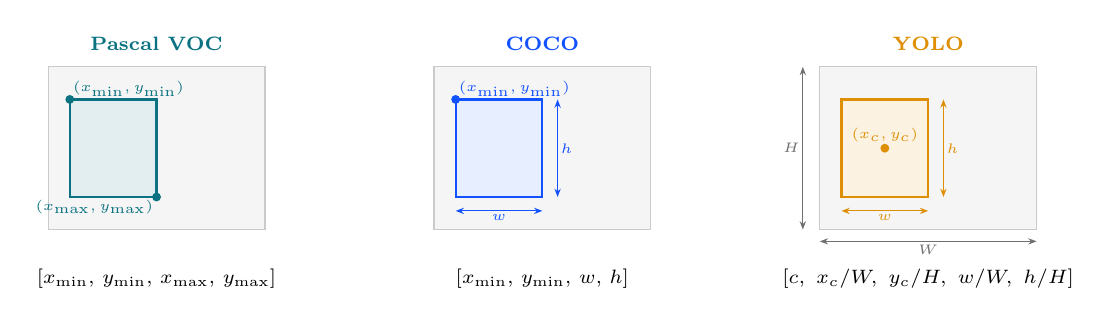
\begin{tikzpicture}[x=0.0043cm, y=-0.0043cm, font=\tiny]
        \tikzset{dim/.style={{Stealth[length=3pt]}-{Stealth[length=3pt]}, thin}}
        % ---------- Pascal VOC ----------
        \begin{scope}
            \fill[dlSoftCloud] (0,0) rectangle (640,480); \draw[dlHairline] (0,0) rectangle (640,480);
            \fill[dlTeal!12] (64,96) rectangle (320,384); \draw[dlTeal, thick] (64,96) rectangle (320,384);
            \fill[dlTeal] (64,96) circle (1.6pt); \fill[dlTeal] (320,384) circle (1.6pt);
            \node[text=dlTeal, anchor=south west, inner sep=1pt] at (64,96) {$(x_{\min},y_{\min})$};
            \node[text=dlTeal, anchor=north east, inner sep=1pt] at (320,384) {$(x_{\max},y_{\max})$};
            \node[anchor=south, font=\scriptsize\bfseries, text=dlTeal] at (320,-20) {Pascal VOC};
            \node[font=\scriptsize] at (320,625) {$[x_{\min},\,y_{\min},\,x_{\max},\,y_{\max}]$};
        \end{scope}
        % ---------- COCO ----------
        \begin{scope}[xshift=4.9cm]
            \fill[dlSoftCloud] (0,0) rectangle (640,480); \draw[dlHairline] (0,0) rectangle (640,480);
            \fill[dlBlue!10] (64,96) rectangle (320,384); \draw[dlBlue, thick] (64,96) rectangle (320,384);
            \fill[dlBlue] (64,96) circle (1.6pt);
            \node[text=dlBlue, anchor=south west, inner sep=1pt] at (64,96) {$(x_{\min},y_{\min})$};
            \draw[dim, dlBlue] (64,425) -- (320,425) node[midway, below, inner sep=1pt] {$w$};
            \draw[dim, dlBlue] (365,96) -- (365,384) node[midway, right, inner sep=1pt] {$h$};
            \node[anchor=south, font=\scriptsize\bfseries, text=dlBlue] at (320,-20) {COCO};
            \node[font=\scriptsize] at (320,625) {$[x_{\min},\,y_{\min},\,w,\,h]$};
        \end{scope}
        % ---------- YOLO ----------
        \begin{scope}[xshift=9.8cm]
            \fill[dlSoftCloud] (0,0) rectangle (640,480); \draw[dlHairline] (0,0) rectangle (640,480);
            \fill[dlOrange!12] (64,96) rectangle (320,384); \draw[dlOrange, thick] (64,96) rectangle (320,384);
            \fill[dlOrange] (192,240) circle (1.6pt);
            \node[text=dlOrange, anchor=south, inner sep=2pt] at (192,240) {$(x_c,y_c)$};
            \draw[dim, dlOrange] (64,425) -- (320,425) node[midway, below, inner sep=1pt] {$w$};
            \draw[dim, dlOrange] (365,96) -- (365,384) node[midway, right, inner sep=1pt] {$h$};
            \draw[dim, dlMute] (0,515) -- (640,515) node[midway, below, inner sep=1pt] {$W$};
            \draw[dim, dlMute] (-50,0) -- (-50,480) node[midway, left, inner sep=1pt] {$H$};
            \node[anchor=south, font=\scriptsize\bfseries, text=dlOrange] at (320,-20) {YOLO};
            \node[font=\scriptsize] at (320,625) {$[c,\ x_c/W,\ y_c/H,\ w/W,\ h/H]$};
        \end{scope}
    \end{tikzpicture}
    \end{center}

    \vspace{-6pt}
    \begin{center}
    \scriptsize\setlength{\tabcolsep}{5pt}
    \begin{tabular}{llll}
        \toprule
         & \textbf{Pascal VOC} & \textbf{COCO} & \textbf{YOLO} \\
        \midrule
        Parameter & 2 sudut (\texttt{xyxy}) & sudut kiri-atas + ukuran (\texttt{xywh}) & pusat + ukuran (\texttt{cxcywh}) \\
        Satuan & piksel & piksel & \textbf{relatif} $[0,1]$ (dibagi $W, H$) \\
        Berkas & 1 XML per citra & 1 JSON per split & 1 \texttt{.txt} per citra \\
        Pemakai & target torchvision & pycocotools (mAP) & Ultralytics \\
        \bottomrule
    \end{tabular}
    \end{center}
    {\scriptsize\color{dlMute} Titik asal $(0,0)$ di \textbf{kiri-atas} citra, sumbu $y$ ke bawah (sama untuk ketiganya).}
\end{frame}

%------------------------------------------------
\begin{frame}
    \frametitle{Contoh Konversi Antar Format}
    \framesubtitle{Box yang Sama, Tiga Cara Menulis}
    \footnotesize

    \begin{columns}[T]
        \column{0.46\textwidth}
        \begin{exampleblock}{Contoh: citra $640\times480$, kelas 0}
            \begin{tabular}{@{}ll@{}}
                Pascal VOC & \texttt{64, 96, 320, 384} \\
                COCO & \texttt{64, 96, 256, 288} \\
                YOLO & \texttt{0 0.300 0.500 0.400 0.600} \\
            \end{tabular}
        \end{exampleblock}
        \vspace{0.1cm}
        $w = 320-64 = 256$, \quad $h = 384-96 = 288$\\[2pt]
        $x_c = \tfrac{64+320}{2} = 192 \;\Rightarrow\; 192/640 = 0{,}3$\\[2pt]
        $y_c = \tfrac{96+384}{2} = 240 \;\Rightarrow\; 240/480 = 0{,}5$\\[2pt]
        $w/W = 256/640 = 0{,}4$, \quad $h/H = 288/480 = 0{,}6$

        \column{0.50\textwidth}
        \begin{block}{Rumus konversi dari \texttt{xyxy}}
            COCO: $w=x_{\max}-x_{\min}$, \ $h=y_{\max}-y_{\min}$\\[2pt]
            YOLO: $\hat x_c=\tfrac{x_{\min}+x_{\max}}{2W}$, \ $\hat y_c=\tfrac{y_{\min}+y_{\max}}{2H}$\\[2pt]
            \phantom{YOLO:} $\hat w=\tfrac{w}{W}$, \ $\hat h=\tfrac{h}{H}$\\[2pt]
            Balik: $x_{\min}=(\hat x_c-\tfrac{\hat w}{2})\,W$, \ $y_{\min}=(\hat y_c-\tfrac{\hat h}{2})\,H$
        \end{block}
        \textbf{Jebakan umum:}
        \begin{itemize}
            \item \textbf{Salah baca format:} box COCO di atas dibaca sebagai \texttt{xyxy} $\Rightarrow$ IoU dengan box asli hanya \textbf{0,5}, padahal model benar.
            \item \textbf{Resize:} label VOC/COCO ikut diskalakan; label YOLO tetap (kecuali crop/padding).
            \item Anotasi VOC asli berindeks piksel mulai 1.
        \end{itemize}
    \end{columns}
\end{frame}

%------------------------------------------------
\begin{frame}[fragile]
    \frametitle{Berkas Anotasi \& Konversi di Python}
    \framesubtitle{Box yang Sama dalam Tiga Berkas}
    \footnotesize

    \begin{columns}[T]
        \column{0.44\textwidth}
        {\scriptsize\textbf{\color{dlTeal}Pascal VOC} --- \texttt{Annotations/img001.xml}}
\begin{lstlisting}[style=py, language={}]
<object>
  <name>cat</name>
  <bndbox>
    <xmin>64</xmin>  <ymin>96</ymin>
    <xmax>320</xmax> <ymax>384</ymax>
  </bndbox>
</object>
\end{lstlisting}
        {\scriptsize\textbf{\color{dlBlue}COCO} --- \texttt{annotations/instances\_train.json}}
\begin{lstlisting}[style=py, language={}]
"annotations": [{"id": 1, "image_id": 1,
  "category_id": 17, "iscrowd": 0,
  "bbox": [64, 96, 256, 288]}]
\end{lstlisting}
        {\scriptsize\textbf{\color{dlOrange}YOLO} --- \texttt{labels/img001.txt}}
\begin{lstlisting}[style=py, language={}]
0 0.300 0.500 0.400 0.600
\end{lstlisting}

        \column{0.52\textwidth}
\begin{lstlisting}[style=py]
import torch
from torchvision.ops import box_convert

W, H = 640, 480
voc  = torch.tensor([[64., 96., 320., 384.]])  # xyxy
coco = box_convert(voc, "xyxy", "xywh")
# tensor([[ 64.,  96., 256., 288.]])
cxcy = box_convert(voc, "xyxy", "cxcywh")
yolo = cxcy / torch.tensor([W, H, W, H])
# tensor([[0.3000, 0.5000, 0.4000, 0.6000]])
\end{lstlisting}
        \begin{itemize}
            \item \texttt{box\_convert} bekerja dalam piksel; normalisasi YOLO dilakukan manual.
            \item Albumentations \texttt{BboxParams(format=...)}: box ikut berubah saat augmentasi.
            \item Kelas: COCO \texttt{category\_id} (kucing $=17$); YOLO indeks mulai 0.
        \end{itemize}
    \end{columns}
\end{frame}

%------------------------------------------------
\begin{frame}
    \frametitle{Bounding Box \& Intersection over Union}
    \framesubtitle{Mengukur Ketepatan Lokalisasi}
    \footnotesize

    \begin{columns}[T]
        \column{0.44\textwidth}
        \begin{center}
        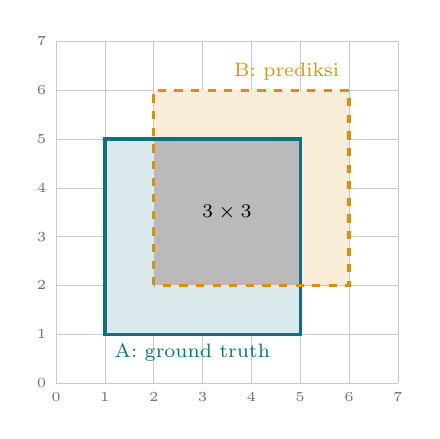
\begin{tikzpicture}[scale=0.62]
            \draw[step=1, dlHairline, very thin] (0,0) grid (7,7);
            \foreach \t in {0,...,7} {\node[font=\tiny, text=dlMute, below] at (\t,0) {\t}; \node[font=\tiny, text=dlMute, left] at (0,\t) {\t};}
            \fill[dlTeal!15] (1,1) rectangle (5,5);
            \fill[dlOrange!15] (2,2) rectangle (6,6);
            \fill[dlCharcoal!35] (2,2) rectangle (5,5);
            \draw[dlTeal, very thick] (1,1) rectangle (5,5);
            \draw[dlOrange, very thick, dashed] (2,2) rectangle (6,6);
            \node[font=\scriptsize, text=dlTeal, anchor=north west] at (1,1) {A: ground truth};
            \node[font=\scriptsize, text=dlOrange, anchor=south east] at (6,6) {B: prediksi};
            \node[font=\scriptsize] at (3.5,3.5) {$3\times3$};
        \end{tikzpicture}
        \end{center}

        \column{0.52\textwidth}
        \textbf{Box} dalam format \texttt{xyxy} (Pascal VOC) + label kelas + skor keyakinan.
        \begin{block}{Intersection over Union}
            $$\text{IoU}(A,B)=\frac{|A\cap B|}{|A\cup B|}\in[0,1]$$
        \end{block}
        \begin{exampleblock}{Contoh: A $=(1,1,5,5)$, B $=(2,2,6,6)$}
            Irisan $=3\times3=9$, gabungan $=16+16-9=23$\\
            $\text{IoU}=9/23\approx\mathbf{0{,}39}$ $<0{,}5$ $\Rightarrow$ dihitung \textbf{salah (FP)} pada ambang 0,5.
        \end{exampleblock}
    \end{columns}
\end{frame}

%------------------------------------------------
\begin{frame}
    \frametitle{NMS \& Metrik mAP}
    \framesubtitle{Membersihkan Duplikat, Lalu Mengukur}
    \footnotesize

    \begin{columns}[T]
        \column{0.48\textwidth}
        \begin{block}{Non-Maximum Suppression (per kelas)}
            \begin{enumerate}
                \item Urutkan box berdasarkan skor.
                \item Ambil box skor tertinggi $\to$ simpan.
                \item Buang box lain dengan IoU $>$ ambang (mis. 0,5) terhadap box tersebut.
                \item Ulangi sampai tidak ada box tersisa.
            \end{enumerate}
        \end{block}
        {\scriptsize\color{dlMute} Detektor menghasilkan ratusan box yang tumpang tindih untuk satu objek; NMS menyisakan satu.}

        \column{0.48\textwidth}
        \textbf{Evaluasi deteksi:}
        $$\text{Precision}=\frac{TP}{TP+FP},\qquad \text{Recall}=\frac{TP}{TP+FN}$$
        \begin{itemize}
            \item Prediksi $=$ TP bila IoU $\ge$ ambang \& kelas benar.
            \item \textbf{AP}: luas di bawah kurva precision--recall satu kelas.
            \item \textbf{mAP}: rata-rata AP seluruh kelas.
            \item \textbf{mAP@0,5} (PASCAL VOC) vs \textbf{mAP@[0,5:0,95]} (COCO: rata-rata 10 ambang IoU, lebih ketat).
        \end{itemize}
    \end{columns}
\end{frame}

%------------------------------------------------
\begin{frame}
    \frametitle{Detektor Dua Tahap: Keluarga R-CNN}
    \framesubtitle{Usulkan Region, Lalu Klasifikasikan}
    \footnotesize

    \begin{center}
    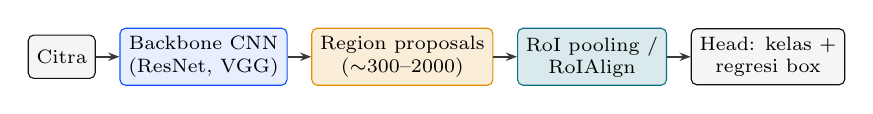
\begin{tikzpicture}[node distance=0.3cm]
        \node[lyr] (img) {Citra};
        \node[lyrB, right=of img] (bb) {Backbone CNN\\(ResNet, VGG)};
        \node[lyrO, right=of bb] (rpn) {Region proposals\\($\sim$300--2000)};
        \node[lyrT, right=of rpn] (roi) {RoI pooling /\\RoIAlign};
        \node[lyr, right=of roi] (head) {Head: kelas +\\regresi box};
        \draw[arr] (img) -- (bb); \draw[arr] (bb) -- (rpn); \draw[arr] (rpn) -- (roi); \draw[arr] (roi) -- (head);
    \end{tikzpicture}
    \end{center}
    \vspace{-2pt}
    \begin{center}
    \scriptsize
    \begin{tabular}{llll}
        \toprule
        \textbf{Model} & \textbf{Sumber proposal} & \textbf{Ide kunci} & \textbf{Kecepatan} \\
        \midrule
        R-CNN (2014) & Selective search & CNN dijalankan \textbf{per region} ($\sim$2000$\times$) & $\sim$47 s/citra \\
        Fast R-CNN (2015) & Selective search & CNN \textbf{sekali} per citra + RoI pooling & $\sim$2 s/citra \\
        Faster R-CNN (2015) & \textbf{Region Proposal Network} & Proposal dipelajari dari \textit{anchor boxes} & $\sim$0,2 s/citra \\
        \bottomrule
    \end{tabular}
    \end{center}
    \vspace{0.1cm}
    \begin{itemize}
        \item \textbf{Anchor}: box acuan berbagai skala \& rasio di tiap lokasi feature map; RPN memprediksi \textit{objectness} + pergeseran box.
        \item Akurat, terutama untuk objek kecil, namun lebih lambat karena dua tahap.
    \end{itemize}
\end{frame}

%------------------------------------------------
\begin{frame}
    \frametitle{Detektor Satu Tahap: YOLO}
    \framesubtitle{You Only Look Once (2016)}
    \footnotesize

    \begin{columns}[T]
        \column{0.36\textwidth}
        \begin{center}
        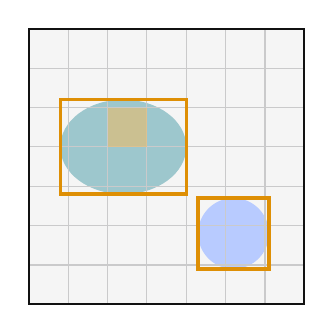
\begin{tikzpicture}[scale=0.5]
            \fill[dlSoftCloud] (0,0) rectangle (7,7);
            \fill[dlTeal!40] (2.4,4.0) ellipse (1.6 and 1.2);
            \fill[dlBlue!30] (5.2,1.8) circle (0.9);
            \draw[step=1, dlHairline] (0,0) grid (7,7);
            \fill[dlOrange!60, opacity=0.6] (2,4) rectangle (3,5);
            \draw[dlOrange, very thick] (0.8,2.8) rectangle (4.0,5.2);
            \draw[dlOrange, very thick] (4.3,0.9) rectangle (6.1,2.7);
            \draw[dlInk, thick] (0,0) rectangle (7,7);
        \end{tikzpicture}
        \end{center}
        {\scriptsize\color{dlMute} Sel oranye memuat pusat objek $\Rightarrow$ sel itu yang bertanggung jawab memprediksinya.}

        \column{0.60\textwidth}
        \begin{block}{Deteksi sebagai satu masalah regresi}
            Citra dibagi grid $S\times S$. Tiap sel memprediksi $B$ box $(x,y,w,h,\text{conf})$ dan $C$ probabilitas kelas:
            $$\text{output} = S\times S\times(5B+C) = 7\times7\times30 \quad (\text{VOC: } B{=}2, C{=}20)$$
        \end{block}
        \begin{itemize}
            \item \textbf{Satu forward pass}, tanpa tahap proposal $\Rightarrow$ $\sim$45 FPS (real-time) pada YOLOv1.
            \item Versi awal lemah pada objek kecil \& berdempetan; versi modern (YOLOv5--v11) memakai anchor/anchor-free, FPN, dan backbone CNN efisien.
            \item Trade-off umum: \textbf{satu tahap = cepat}, \textbf{dua tahap = akurat}.
        \end{itemize}
    \end{columns}
\end{frame}

%------------------------------------------------
\begin{frame}
    \frametitle{Semantic Segmentation: FCN \& U-Net}
    \framesubtitle{Arsitektur Encoder--Decoder}
    \footnotesize

    \begin{columns}[T]
        \column{0.54\textwidth}
        \begin{center}
        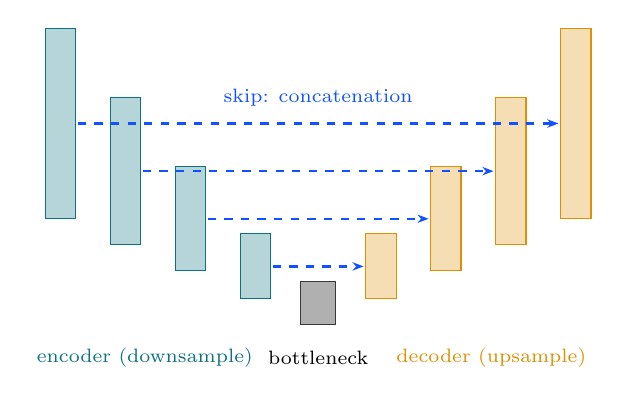
\begin{tikzpicture}[x=0.55cm,y=0.55cm]
            % encoder
            \foreach \i/\h in {0/4.4, 1/3.4, 2/2.4, 3/1.5} {
                \fill[dlTeal!30, draw=dlTeal] (\i*1.5, 5-\i*1.1-\h/2) rectangle ++(0.7,\h);
            }
            \fill[dlCharcoal!40, draw=dlCharcoal] (5.9, 0.35) rectangle ++(0.8,1.0);
            % decoder
            \foreach \i/\h in {3/1.5, 2/2.4, 1/3.4, 0/4.4} {
                \fill[dlOrange!30, draw=dlOrange] (12.6-\i*1.5-0.7, 5-\i*1.1-\h/2) rectangle ++(0.7,\h);
            }
            % skip connections
            \foreach \i in {0,1,2,3} {
                \draw[-{Stealth[length=4pt]}, dlBlue, thick, dashed] (\i*1.5+0.75, 5-\i*1.1) -- (12.6-\i*1.5-0.75, 5-\i*1.1);
            }
            \node[font=\scriptsize, text=dlTeal] at (2.3,-0.4) {encoder (downsample)};
            \node[font=\scriptsize, text=dlOrange] at (10.3,-0.4) {decoder (upsample)};
            \node[font=\scriptsize, text=dlBlue] at (6.3,5.6) {skip: concatenation};
            \node[font=\scriptsize] at (6.3,-0.4) {bottleneck};
        \end{tikzpicture}
        \end{center}

        \column{0.42\textwidth}
        \textbf{FCN (Long et al., 2015)}
        \begin{itemize}
            \item Ganti FC dengan conv $1\times1$ $\Rightarrow$ bisa menerima ukuran input apa pun.
            \item \textit{Upsampling} (transposed conv) memulihkan resolusi: output $H\times W\times C$.
        \end{itemize}
        \textbf{U-Net (Ronneberger et al., 2015)}
        \begin{itemize}
            \item Encoder mengompres konteks, decoder memulihkan detail.
            \item \textbf{Skip concatenation} mengirim fitur resolusi tinggi dari encoder ke decoder $\Rightarrow$ batas tajam.
            \item Standar de facto citra medis \& model difusi.
        \end{itemize}
    \end{columns}
\end{frame}

%------------------------------------------------
\begin{frame}
    \frametitle{Instance Segmentation: Mask R-CNN}
    \framesubtitle{Satu Backbone, Banyak Head}
    \footnotesize

    \begin{columns}[T]
        \column{0.48\textwidth}
        \begin{block}{Mask R-CNN (He et al., 2017)}
            Faster R-CNN + \textbf{cabang mask}: untuk setiap RoI, prediksi mask biner $28\times28$ per kelas, paralel dengan kelas \& box.
        \end{block}
        \begin{itemize}
            \item \textbf{RoIAlign}: interpolasi bilinear tanpa pembulatan koordinat (RoI pooling membulatkan $\Rightarrow$ mask bergeser).
            \item Loss total: $L = L_{cls} + L_{box} + L_{mask}$.
        \end{itemize}

        \column{0.48\textwidth}
        \textbf{Benang merah hari ini:}
        \begin{center}
        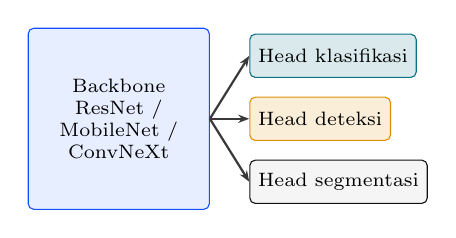
\begin{tikzpicture}[node distance=0.22cm and 0.5cm]
            \node[lyrB, minimum width=2.3cm, minimum height=2.3cm] (bb) {Backbone\\ResNet /\\MobileNet /\\ConvNeXt};
            \node[lyrT, right=of bb, yshift=0.8cm] (h1) {Head klasifikasi};
            \node[lyrO, right=of bb] (h2) {Head deteksi};
            \node[lyr, right=of bb, yshift=-0.8cm] (h3) {Head segmentasi};
            \draw[arr] (bb.east) -- (h1.west); \draw[arr] (bb.east) -- (h2.west); \draw[arr] (bb.east) -- (h3.west);
        \end{tikzpicture}
        \end{center}
        {\scriptsize\color{dlMute} Arsitektur yang dipelajari di Bagian 1--4 adalah ``mesin fitur'' untuk seluruh tugas computer vision; \texttt{torchvision} menyediakan \texttt{fasterrcnn\_resnet50\_fpn}, \texttt{maskrcnn\_resnet50\_fpn}, dan \texttt{deeplabv3\_resnet50}.}
    \end{columns}
\end{frame}

%================================================
\section*{Penutup}

%------------------------------------------------
\begin{frame}
    \frametitle{Ringkasan Pertemuan 5}
    \framesubtitle{Capaian Pembelajaran (RPS IF25-40401)}
    \footnotesize

    \begin{enumerate}
        \item \textbf{AlexNet $\to$ VGG:} ReLU, dropout, augmentasi, GPU; lalu tumpukan $3\times3$ seragam (RF sama, bobot $18C^2$ vs $25C^2$).
        \item \textbf{Efisiensi awal:} konvolusi $1\times1$ dan GAP (GoogLeNet) membuang FC raksasa yang memakan $\sim$90\% parameter VGG.
        \item \textbf{ResNet:} $H(x)=F(x)+x$ mengatasi \textit{degradation problem}; suku $+1$ menjaga aliran gradien; bottleneck $1\times1$--$3\times3$--$1\times1$.
        \item \textbf{MobileNet:} depthwise + pointwise memangkas biaya menjadi $\tfrac1N+\tfrac1{D_K^2}$ ($\sim$9$\times$ lebih hemat); EfficientNet menskalakan $d, w, r$ bersamaan.
        \item \textbf{ConvNeXt:} resep training modern, patchify stem, depthwise $7\times7$, inverted bottleneck, GELU, LayerNorm $\Rightarrow$ CNN murni menyaingi Swin.
        \item \textbf{Deteksi \& segmentasi:} format box (VOC/COCO/YOLO), IoU, NMS, mAP; dua tahap (Faster R-CNN) vs satu tahap (YOLO); encoder--decoder (FCN, U-Net); Mask R-CNN.
    \end{enumerate}

    \vspace{0.1cm}
    {\scriptsize\color{dlMute}\textbf{Pertemuan 6 --- Studio Proyek 2: Fine-tuning CNN Pretrained.} Bawa laptop, siapkan akun Kaggle/Colab dengan GPU; kelompok 2 orang.}
\end{frame}

%------------------------------------------------
\begin{frame}
    \frametitle{Latihan Mandiri (Tugas Terstruktur)}
    \framesubtitle{TT 3$\times$60$'$ --- Hitung dengan Tangan}
    \footnotesize

    \begin{enumerate}
        \item \textbf{Blok 3 VGG-16:} input $56\times56\times128$, tiga conv $3\times3$ 256 filter ($P=1$) lalu max-pool $2\times2$. Hitung ukuran output dan total parameter (termasuk bias).
        \item \textbf{ResNet pada 512 kanal:} bandingkan jumlah bobot basic block ($2\times$ conv $3\times3$, 512 kanal) dengan bottleneck ($1\times1$ 128, $3\times3$ 128, $1\times1$ 512). Berapa kali lipat penghematannya?
        \item \textbf{Depthwise separable $5\times5$:} dengan $M=N=256$, turunkan rasio biaya terhadap konvolusi standar. Mengapa penghematannya lebih besar dibanding kernel $3\times3$?
        \item \textbf{IoU:} ground truth $(10,20,50,80)$ dan prediksi $(30,40,70,90)$ dalam format $(x_1,y_1,x_2,y_2)$. Hitung IoU; apakah TP pada ambang 0,5? Tulis juga prediksi dalam format COCO dan YOLO (citra $100\times100$).
        \item \textbf{Analisis tabel perbandingan:} pilih dua backbone untuk aplikasi deteksi penyakit daun di ponsel petani, dan justifikasi dengan angka params, GFLOPs, dan top-1.
    \end{enumerate}
    \vspace{0.1cm}
    {\scriptsize\color{dlMute} Kumpulkan jawaban tulisan tangan (foto/PDF) melalui LMS sebelum Pertemuan 6.}
\end{frame}

%------------------------------------------------
\begin{frame}
    \frametitle{Referensi (1/3)}
    \framesubtitle{Arsitektur Klasifikasi}
    \scriptsize
    \begin{thebibliography}{9}
        \bibitem{alexnet} A. Krizhevsky, I. Sutskever, G. Hinton. ImageNet Classification with Deep Convolutional Neural Networks. \textit{NeurIPS}, 2012.
        \bibitem{vgg} K. Simonyan, A. Zisserman. Very Deep Convolutional Networks for Large-Scale Image Recognition. \textit{ICLR}, 2015.
        \bibitem{googlenet} C. Szegedy et al. Going Deeper with Convolutions. \textit{CVPR}, 2015.
        \bibitem{bn} S. Ioffe, C. Szegedy. Batch Normalization: Accelerating Deep Network Training by Reducing Internal Covariate Shift. \textit{ICML}, 2015.
        \bibitem{resnet} K. He, X. Zhang, S. Ren, J. Sun. Deep Residual Learning for Image Recognition. \textit{CVPR}, 2016.
        \bibitem{densenet} G. Huang, Z. Liu, L. van der Maaten, K. Weinberger. Densely Connected Convolutional Networks. \textit{CVPR}, 2017.
        \bibitem{mobilenet} A. Howard et al. MobileNets: Efficient Convolutional Neural Networks for Mobile Vision Applications. \textit{arXiv:1704.04861}, 2017.
        \bibitem{mobilenetv2} M. Sandler et al. MobileNetV2: Inverted Residuals and Linear Bottlenecks. \textit{CVPR}, 2018.
        \bibitem{efficientnet} M. Tan, Q. Le. EfficientNet: Rethinking Model Scaling for Convolutional Neural Networks. \textit{ICML}, 2019.
    \end{thebibliography}
\end{frame}

%------------------------------------------------
\begin{frame}
    \frametitle{Referensi (2/3)}
    \framesubtitle{ConvNeXt, Deteksi \& Segmentasi}
    \scriptsize
    \begin{thebibliography}{9}
        \bibitem{convnext} Z. Liu et al. A ConvNet for the 2020s. \textit{CVPR}, 2022.
        \bibitem{rcnn} R. Girshick et al. Rich Feature Hierarchies for Accurate Object Detection and Semantic Segmentation. \textit{CVPR}, 2014.
        \bibitem{fastrcnn} R. Girshick. Fast R-CNN. \textit{ICCV}, 2015.
        \bibitem{fasterrcnn} S. Ren, K. He, R. Girshick, J. Sun. Faster R-CNN: Towards Real-Time Object Detection with Region Proposal Networks. \textit{NeurIPS}, 2015.
        \bibitem{yolo} J. Redmon et al. You Only Look Once: Unified, Real-Time Object Detection. \textit{CVPR}, 2016.
        \bibitem{fcn} J. Long, E. Shelhamer, T. Darrell. Fully Convolutional Networks for Semantic Segmentation. \textit{CVPR}, 2015.
        \bibitem{unet} O. Ronneberger, P. Fischer, T. Brox. U-Net: Convolutional Networks for Biomedical Image Segmentation. \textit{MICCAI}, 2015.
        \bibitem{maskrcnn} K. He, G. Gkioxari, P. Dollár, R. Girshick. Mask R-CNN. \textit{ICCV}, 2017.
    \end{thebibliography}
\end{frame}

%------------------------------------------------
\begin{frame}
    \frametitle{Referensi (3/3)}
    \framesubtitle{Dataset \& Pustaka}
    \scriptsize
    \begin{thebibliography}{9}
        \bibitem{voc} M. Everingham, L. Van Gool, C. Williams, J. Winn, A. Zisserman. The PASCAL Visual Object Classes (VOC) Challenge. \textit{IJCV}, 2010.
        \bibitem{coco} T.-Y. Lin et al. Microsoft COCO: Common Objects in Context. \textit{ECCV}, 2014.
        \bibitem{tv} PyTorch Team. torchvision.models --- Models and pre-trained weights. \url{https://pytorch.org/vision/stable/models.html}
        \bibitem{tvops} PyTorch Team. torchvision.ops.box\_convert. \url{https://pytorch.org/vision/stable/generated/torchvision.ops.box_convert.html}
        \bibitem{ultra} Ultralytics. YOLO Dataset Format (Object Detection). \url{https://docs.ultralytics.com/datasets/detect/}
    \end{thebibliography}
\end{frame}

%------------------------------------------------
%	CLOSING SLIDE
%------------------------------------------------
\begin{frame}[plain]
  \begin{beamercolorbox}[wd=\paperwidth,ht=\paperheight,sep=1.5cm]{palette primary}
    \vspace{1.5cm}
    {\scriptsize\bfseries\color{dlMute}IF25-40401 · DEEP LEARNING}\\[0.4cm]
    {\Huge\bfseries Terima Kasih}\\[0.4cm]
    {\small Pertemuan Berikutnya: Studio Proyek 2 --- Fine-tuning CNN Pretrained pada ImageNet}\\[1.0cm]
    \vfill
    {\scriptsize\textbf{Tim Dosen Deep Learning} · Institut Teknologi Sumatera (ITERA)}
  \end{beamercolorbox}
\end{frame}

\end{document}
